\begin{refsection}
\hypertarget{numbers}{%
\chapter{Number systems}\label{chap-numbers}}

\hypertarget{introduction}{%
\section{Introduction}}

 In order to understand problems about number systems, we firstly need to understand the concept of base and the characteristics of such systems.

In Romanian, for example, the number 432 is written \cmubdata{patru sute treizeci și doi}. It can be segmented into morphemes as follows: \cmubdata{patru} (\texttr{four}) \cmubdata{sute} (\texttr{hundreds}) \cmubdata{trei} (\texttr{three})-\cmubdata{zeci} (\texttr{tens}) \cmubdata{și} (\texttr{and}) \cmubdata{doi} (\texttr{two}), and each morpheme has a well defined role. The morphemes \cmubdata{patru}  (\texttr{four}), \cmubdata{trei} (\texttr{three}), \cmubdata{doi} (\texttr{two}) represent the \textit{digits}, the basic units, while the morphemes \cmubdata{sute} (\texttr{hundreds}) and \cmubdata{zeci} (\texttr{tens}) represent the \textit{orders}, i.e., some greater base words. Finally, the morpheme \cmubdata{și} (\texttr{and}) denotes addition. Since in this case the orders are 10 and 100 (10\textsuperscript{1}, 10\textsuperscript{2}), we are talking about a base-10 (or decimal) system.

Moreover, word order plays an important role, together with the way in which the multiplication and the addition are marked. Returning to the example \cmubdata{patru sute treizeci și doi}, we can deduce the following:

\begin{itemize}
    \item the general order is from big to small (we first write the hundreds, then the tens and finally the units);
    \item the multiplier is placed before the order (thus, we write \cmubdata{patru sute} and not \cmubdata{*sute patru});
    \item the morpheme for \texttr{tens} is written as part of the same word with its multiplier (\cmubdata{treizeci}, not \cmubdata{*trei zeci});
    \item the tens are separated from the units by the word \cmubdata{și}.
\end{itemize}

 There is also a simpler method to show all of these rules, by writing the general structure of the number:

\exrule{100X + 10Y + Z = X \cmubdata{sute} Y-\cmubdata{zeci și} Z}

 This rule combines all four rules from above, showing the sequence of the orders (hundreds, tens, units), the position of the multiplier (as a separate word before the hundreds and combined with the ending \cmubdata{zeci} for tens), as well as the morpheme \cmubdata{și} added between tens and units.

Although base 10 is the most common base and most languages use it, there are also other bases, among which the most common are base 6 and base 20. Less common, but occurring in a reasonable number of languages are bases 4, 5, 12, and 60, while bases 7, 9, 11, and 13 are extremely rare (at the moment, no known natural language uses them), so that, in linguistics problems, we can assume from the beginning that the system is highly unlikely to have the bases 7, 9, 11, 13.

A special category of bases is 22–28, which are found in languages whose number system is based on body parts, such as Oksapmin or Kaugel.

In order to better understand the concept of base, let us consider how the numbers 10, 25, and 100 would be written in a base-6 system. Since the base is 6, the orders are 6 (6\textsuperscript{1}), 36 (6\textsuperscript{2}), 216 (6\textsuperscript{3}), and so on. Therefore, the number 10 will be written as $6+4$ (or $4+6$, depending on the word order), number 25 will be written as $(4\times6)+1$, while 100 will be written as $(2\times36)+(4\times6)+4$.

So, in problems involving number systems, there are two important characteristics:

\begin{enumerate}[label = (\arabic*)]
    \item word order (or direction): big-to-small or small-to-big or a mixture;
    \item the way in which addition and multiplication are marked (or whether they are not overtly marked).
\end{enumerate}

In terms of (1), remember that it is not necessary that the word order is strictly ascending or descending, and there can also be exceptions. For example, in German, 432 is written \cmubdata{vierhundertzweiunddreißig} (\cmubdata{vier-hundert-zwei-und-drei-ßig} = 4-\texttr{hundreds}-2-\texttr{plus}-3-\texttr{tens}), so the order is hundreds-units-tens. In terms of (2), note that in French, for example, in the number 2,510 (\cmubdata{deux mille cinq cent dix} = \texttr{two} - \texttr{thousand} - \texttr{five} - \texttr{hundred} - \texttr{ten}), both the addition and the multiplication are implicit and as such, if the digit is placed before the order, it gets multiplied, while addition occurs every time after the order (e.g., 2,510 can be written as $(2\times1000)+(5\times100)+10$). Moreover, if the addition or multiplication is marked, this will be done using a rather pervasive morpheme, word, or group of words.

\begin{problem}{\langnameQuenya}{\nameRDinca}{\LOYear{\RoLOAbbr}{2013}}
Here are some Quenya numbers:
\begin{center}
    \begin{tabular}{lr@{\qquad\qquad}lr}
         \pbsvnum{neldë}{3} & \pbsvnum{enquë yucainen}{26} \\
         \pbsvnum{canta}{4} & \pbsvnum{minë nelcainen}{31} \\
         \pbsvnum{lempë}{5} & \pbsvnum{cancainen}{40} \\
         \pbsvnum{otso}{7} & \pbsvnum{atta tolcainen}{82} \\
         \pbsvnum{tolto}{8} & \pbsvnum{atta tolcainen tuxa}{182} \\
         \pbsvnum{nelcëa}{13} & \pbsvnum{nertë nelcainen lemtuxa}{539} \\
         \pbsvnum{encëa}{16} & \pbsvnum{}{} \\
    \end{tabular}
\end{center}

\begin{assgts}
\item \taskWriteNumbers:
\begin{multicols}{2}
\begin{enumerate}[label = \alph*.]
    \item \cmubdata{tolcëa}
    \item \cmubdata{enquë cancainen}
    \item \cmubdata{cancainen neltuxa}
    \item \cmubdata{lempë tolcainen}
    \item \cmubdata{tuxa}
    \blankitem
\end{enumerate}
\end{multicols}
\item \taskWriteIn{\langnameQuenya}: 1, 70, 192, 385.
\end{assgts}
\end{problem}

\begin{mysolution}

 We notice that numbers 13 and 16 both end in the suffix \cmubdata{-cëa}, while numbers bigger than 26 have a different structure. Thus, comparing the words for 3 and 13, we can assume it is a base-10 language and that numbers $10$ $+$ $X$ are written as \cmubdata{X-cëa}. We further notice that in order to form the number 13, only a part of the word for 3 is used (\cmubdata{nel}).

Comparing examples 82 and 182, they differ only by the word \cmubdata{tuxa} placed at the end; therefore, we can deduce that \cmubdata{tuxa} means 100 (which further confirms that the number system for this language is base 10). Moreover, looking at the number 539, we notice that the last word is \cmubdata{lemtuxa}, where \cmubdata{tuxa} = 100, and \cmubdata{lem} is the first part of the number 5. Thus, in this case as well, only a part of the stem of the unit is used. Furthermore, we notice that in the right column, the second word always ends in \cmubdata{cainen}. We can assume that this is the suffix which marks the tens ($10X$), whence we deduce that the word order in Quenya is units-tens-hundreds.

Only based on these observations, we can write the following rules:

\exrule{$10+X$ = $X$′ \cmubdata{-cëa} \quad\quad\quad $100X+10Y+Z$ = $Z$ $Y$′\cmubdata{-cainen} $X$′\cmubdata{-tuxa}}

 By $X$′ and $Y$′ we mean that a different, truncated, form of the word is used.

 Based on these observations, we can create a table with the form of each digit in different contexts:

\begin{table}[H]
    \begin{tabular}{clccc}
    \lsptoprule
    Digit & \multicolumn{1}{c}{$X$} & $10+X$ & $10X$ & $100X$ \\\midrule
    1 & \cmubdata{minë} & & & $\varnothing$ \\
    2 & \cmubdata{atta} & &\cmubdata{yu-} & \\
    3 & \cmubdata{neldë} & \cmubdata{nel-} & \cmubdata{nel-} & \\
    4 & \cmubdata{canta} & & \cmubdata{can-}& \\
    5 & \cmubdata{lempë} & & & \cmubdata{lem-} \\
    6 & \cmubdata{enquë} & \cmubdata{en-} & & \\
    7 & \cmubdata{otso} & & & \\
    8 & \cmubdata{tolto} & & \cmubdata{tol-} & \\
    9 & \cmubdata{nertë} & & & \\
    \lspbottomrule
    \end{tabular}
\end{table}

The four columns represent the form in which the respective digit is used if it represents the units, if it appears with the suffix \cmubdata{-cëa} (meaning $10+X$), if it appears with the suffix \cmubdata{-cainen} ($10X$), or if it appears with the suffix \cmubdata{-tuxa} ($100X$).

We notice that the same form of 3 appears both in the case of $10+X$ and $10X$. Therefore, we deduce that both contexts use the same form. Moreover, we have no reason not to assume that the same form will also be used in the case of hundreds. In order to deduce how that form is constructed, we compare it with the full form in the first column (the units). We notice that the short form (which we designated by $X$′ and $Y$′) represents the first syllable of the unit. The only exception is the digit 2, where the form used for 20 is \cmubdata{yu-}. It appears that in Quenya 1 and 2 are irregular and have different forms in different contexts. This is not uncommon cross-linguistically. 

Thus, we can solve the tasks and write the rules.

\rules Digits are single words. In compound words, only the stem of the digit is used, which is represented by the first syllable (in the notation below, $X$′ is the stem/first syllable of $X$). The digit 2 has a special form, \cmubdata{yu-}. Thus:

\exrule{$10+X$ = $X$′\cmubdata{-cëa} \quad\quad\quad $100X+10Y+Z$ = $Z$ $Y$′\cmubdata{-cainen} $X$′\cmubdata{-tuxa}}

\pagebreak
\begin{assgts}
    \item
     \begin{multicols}{5}
        \begin{enumerate}[leftmargin = 1em, label = \alph*.]
            \item 18
            \item 46
            \item 340
            \item 85
            \item 100
        \end{enumerate}
    \end{multicols}
    \item
    \begin{multicols}{2}
    \setlength\columnsep{2em}
        \begin{itemize}[leftmargin = 0em]
            \item[] 1 = \cmubdata{minë}
            \item[] 70 = \cmubdata{otcainen}
            \item[] 192 = \cmubdata{atta nercainen tuxa}
            \item[] 385 = \cmubdata{lempë tolcainen neltuxa}
        \end{itemize}
    \end{multicols}
\end{assgts}

 In situations where the base is unknown, a simple method to get some additional information is to count how many morphemes there are. If in a particular language we count 11 digits, we expect the base to be, most likely, 10 or 12. Usually, this method is just an estimation, and the result should probably be taken with an error margin of ±2 because: (1) it is possible that we misidentified some of the digits, and (2) it is possible that the problem does not feature all the digits or even some digits might have different forms in different contexts. Moreover, it is extremely important that we count only the digits, not other morphemes (such as orders or addition/multiplication markers).

\end{mysolution}
\begin{problem}{\langnameChami}{\nameVNeacsu}{\LOYear{\PLOAbbr}{2022}}
Here are two equalities in Embera Chami:
\begin{center}
\begin{tabular}{@{}cr@{\hskip0.02in}c@{\hskip0.02in}l@{}}
     \eqline{umbea $+$ huasoma kwimane}{omme huasoma omme}
     \eqline{omme huasoma kwimane $+$ huasoma abba}{kwimane huasoma}
\end{tabular}
\end{center}

\begin{assgts}
\item Write the equalities above with numerals.
\item \taskWriteIn{\langnameChami}: 1, 5, 17, 23.
\end{assgts}
\end{problem}

\begin{mysolution}

At first sight, it might seem a very difficult problem without an obvious starting point and with very little information given. Nevertheless, if we check the structure of the numbers, we notice that there are two types: single words or numbers like $X$ \cmubdata{huasoma} $Y$. We can assume that the second type will represent bigger numbers, and that \cmubdata{huasoma} is the base, these numbers representing $X\times \text{\cmubdata{huasoma}} + Y$ (or $Y × \text{\cmubdata{huasoma}} + X$). Moreover, we notice that the same word can represent both $X$ and $Y$, therefore $X$ and $Y$ are the slots where the digits are placed. Based on these rules, we can try to count the number of digits that occur in the problem, and we notice that there are only four (\cmubdata{umbea}, \cmubdata{kwimane}, \cmubdata{omme}, \cmubdata{abba}). Moreover, they have a constant form (there are no changes or added or deleted morphemes). We can then assume that the base is 5 and that \cmubdata{huasoma} = 5.

The next thing we need to do is figure out the order of the constituents, i.e., figure out whether $X$ \cmubdata{huasoma} $Y$ means $5X + Y$ or $5Y + X$. Looking at equality (1), we have two cases:


\begin{enumerate}[label = \alph*.]
\begin{multicols}{2}
    \item \cmubdata{huasoma} $X = 5X$
    \item \cmubdata{huasoma} $X = 5+X$
    \end{multicols}
\end{enumerate}


 Assuming case a. is true, eq. (1) becomes:

\exrule{$\text{\cmubdata{umbea}}+5\times\text{\cmubdata{kwimane}} = \text{\cmubdata{omme}}+5\times\text{\cmubdata{omme}}$}

 This seems unlikely, since we know that \cmubdata{umbea} is, most likely, a digit. Thus, if \cmubdata{huasoma kwimane} meant $5X$, then \cmubdata{umbea} $+$ \cmubdata{huasoma kwimane} should be equal to \cmubdata{umbea huasoma kwimane} (i.e., \cmubdata{umbea} $+ 5\times$\cmubdata{kwimane}). Generally, the carryover\footnote{We use the term \textit{carryover} for the following situation: when you add 17 and 19, you add the units first (7 and 9 to get 16) and “carry over”\ the 1 (from 16) to the tens.} is a strong strategy to discover certain digits.

Thus, case b. must be correct, and now we know that \cmubdata{huasoma} $X = 5 + X$, so we can deduce that $X$ \cmubdata{huasoma} $= 5X$ and, extrapolating, $X$ \cmubdata{huasoma} $Y = 5X + Y$.

Moreover, from eq. (1), we see that the number resulting from the addition has the multiplier \cmubdata{omme}. Since this is the result of a sum between a unit and a number like base $+$ $X$, the result can either also be base $+$ $X$ (if there is no carryover) or $2\times$base $+$ $X$ (if there is carryover). Since we know that there is carryover (the number on the right has a multiplier, since it has the structure $5X+Y$), we deduce that \cmubdata{omme} = 2.

If we denote the remaining three digits by $U$, $K$ and $A$ (corresponding to their first letter), we can rewrite the equalities as follows:
\begin{enumerate}[leftmargin = 5em, label = (\arabic*)]
    \item $U+(5+K)=12$
    \item $(10+K)+(5+A)=5K$
\end{enumerate}

 Rearranging equality (1), we get: $U + K = 7$.

Knowing that $U$ and $K$ are digits smaller than $5$ (the base), $U$ and $K$ can only correspond to $3$ and $4$, not necessarily in this order. Thus, $A$ can only be $1$ since it is the only remaining digit. Therefore, \cmubdata{abba} $= 1$.

Replacing this in eq. (2) gives us: $10 + K + 6 = 5K \Leftrightarrow 4K = 16$. So $K = 4$ and, subsequently, $U = 3$.

Thus, the rules are:
\begin{itemize}
    \item 1 = \cmubdata{abba}, 2 = \cmubdata{omme}, 3 = \cmubdata{umbea}, 4 = \cmubdata{kwimane}, 5 = \cmubdata{huasoma};
    \item $5X + Y = X$ \cmubdata{huasoma} $Y$.
\end{itemize}

\begin{solutions}
    \item
    \begin{multicols}{2}
        \begin{enumerate}[label = (\arabic*)]
            \item $3+9=12$
            \item $14+6=20$
        \end{enumerate}
    \end{multicols}
    \item
    \begin{itemize}
        \item[] $1 =$ \cmubdata{abba}
        \item[] $5 =$ \cmubdata{huasoma}
        \item[] $17 = 3\times5+2 =$ \cmubdata{umbea huasoma omme}
        \item[] $23 = 4\times5+3 =$ \cmubdata{kwimane huasoma umbea}
    \end{itemize}
\end{solutions}
\end{mysolution}

\begin{discussion}
For this problem, notice that counting the digits and understanding the structure of the numbers is extremely important for number problems. Moreover, carryovers offer valuable information for problems in which equalities are given, and they can usually be used to infer the digits 2 and 3.

Moreover, it is important to mention that, in order to be able to solve the problem, we need to use the fact that the problem is self-sufficient, otherwise we cannot deduce that the base is 5. Let us consider a base $B$ and the following values for the digits: \cmubdata{omme} $= 2$, \cmubdata{kwimane} $= 4$, \cmubdata{abba} $= B-4$, \cmubdata{umbea} $= B-2$. The equalities become:

\begin{enumerate}[leftmargin = 5em, label = (\arabic*)]
    \item $(B–2) + B + 4 = 2B + 2$
    \item $2B + 4 + (B + (B–4)) = 4B$
\end{enumerate}

 In this case, the two equalities hold, no matter the base (e.g., for base 13 we would get the equalities: (1) $11 + 17 = 28$ and (2) $30 + 22 = 52$). Nevertheless, task (b) asks for the translation of 1, so \cmubdata{abba} needs to be 1 (we know that \cmubdata{umbea} is bigger than \cmubdata{abba}, since $B-4 < B-2$), and if \cmubdata{abba} $= 1 = B-4 \Rightarrow B = 5$.

This is the complete thought process based upon which we deduce the base is 5. However, generally, we expect that the problem features all (or almost all) digits, enabling us to estimate the base based on counting the digits.
\end{discussion}

\begin{problem}{\langnameYupik}{\nameKLow}{\LOYear{\UKLOAbbr}{2017}}
Yup'ik people have an interesting concept when it comes to counting – the words for the numbers can be broken down into meaningful parts which may be related to body parts. For example, the word for 5, \cmubdata{talliman}, means \texttr{arm} and the word for 6, \cmubdata{arvinlegen}, means \texttr{cross over}, as you need to change hands to go on counting. 

The Yup'ik people often include geometry in the border patterns of their traditional garments, called "parkas". One such pattern comes from a $3\times3$ square, as represented below. This is a magic square, constructed by placing the digits 1 to 9 within the cells such that the sum of all the digits in every row, column, and diagonal is the same.
\begin{center}
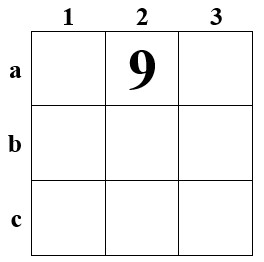
\includegraphics[width = 4cm]{images/Yupik_square.jpg}
\end{center}

To help you fill in the magic square, the following clues are given in Yup'ik.
\textit{Hint:} 294 in Yup'ik is \cmubdata{yuinaat qula cetaman qula cetaman}.

\begin{itemize}
\item Rows:
    \begin{enumerate}[label = \alph*.,nosep]
     \item \cmubdata{Yuinaat yuinaq cetaman qula malruk}
     \item \cmubdata{Yuinaat akimiaq malruk akimiaq malruk}
     \item \cmubdata{Yuinaat yuinaak malruk akimiaq atauciq}
     \end{enumerate}
\item Columns:
    \begin{enumerate}[nosep]
      \item \cmubdata{Yuinaat yuinaq atauciq akimiaq pingayun}
      \item \cmubdata{Yuinaat yuinaak malruk yuinaat malrunglegen qula atauciq}
      \item \cmubdata{Yuinaat qula pingayun akimiaq atauciq}
    \end{enumerate}
\end{itemize}


\begin{assgts}
\item Fill in the numbers missing from the magic square above. One digit is already given (a2 = 9).
\item Write in Yup'ik the number given in the diagonal from top left (the number formed by the digits a1-b2-c3).

\end{assgts}
\end{problem}

\begin{mysolution}

\subsubsection*{1. Solving the magic square}

This is in reality the easiest part. It is known that in a magic square the middle number must be 5 (you can attempt a mathematical proof, it is rather easy), hence b2 = 5. Moreover, it is known that the sum on every row, column and diagonal must be 15. Since on the middle column we already have 9 and 5, we deduce that c2 = 1.

On the first row, we already have the digit 9, so the sum of the other two digits must be 6. We have three possibilities: 5 and 1 (impossible, since 5 is already used), 3 and 3 (impossible, since we cannot repeat digits), or 4 and 2 (this is therefore the only possible option). Therefore, the first row can be either 492 or 294. Since in the introduction we are given the Yup'ik name for 294, which does not appear in the crossword clues (hence, it doesn't appear in the square), we deduce that the first row must be 492, so a1 = 4, a3 = 2.

Since we are told that the sum on the diagonals is also constant (so, 15), we can easily deduce that c1 = 8 and c3 = 6, which makes filling in the rest of the square trivial. In the end we get:

\begin{center}
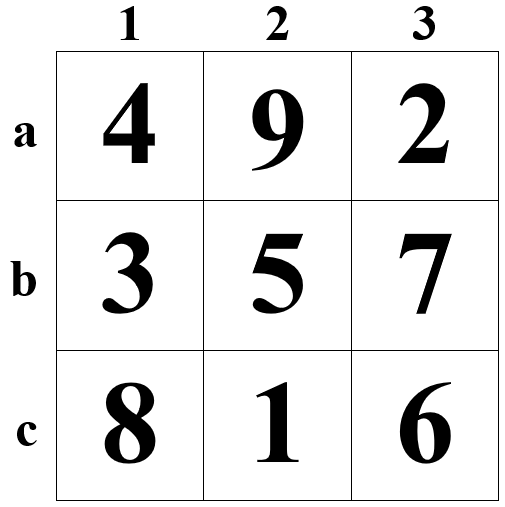
\includegraphics[width = 4cm]{images/Yupik_Square-solved.png}
\end{center}

\subsubsection*{2. Solving the number problem}

 Once the square is filled in, we can extract all the information in a table, transforming the problem into a classic one, in which we are given some numbers spelled out in Yup'ik:

    \begin{longtable}{cl}
    276 & \cmubdata{yuinaat qula pingayun akimiaq atauciq} \\
    294 & \cmubdata{yuinaat qula cetaman qula cetaman} \\
    357 & \cmubdata{yuinaat akimiaq malruk akimiaq malruk} \\
    438 & \cmubdata{yuinaat yuinaq atauciq akimiaq pingayun} \\
    492 & \cmubdata{yuinaat yuinaq cetaman qula malruk} \\
    816 & \cmubdata{yuinaat yuinaak malruk akimiaq atauciq} \\
    951 & \cmubdata{yuinaat yuinaak malruk yuinaat malrunglegen qula atauciq} \\
    \end{longtable}

 The first important observation is based on the last word in every number. We have four types of numbers: ending in \cmubdata{atauciq} (276, 816, 951), ending in \cmubdata{malruk} (357, 492), ending in \cmubdata{cetaman} (294), and ending in \cmubdata{pingayun} (438). Looking closely, one notices that these numbers can be grouped based on their remainder when divided by 5 (i.e., modulo 5). Thus, we can deduce that:

\exrule{\cmubdata{atauciq} = 1, \cmubdata{malruk} = 2, \cmubdata{pingayun} = 3, \cmubdata{cetaman} = 4}

 Replacing these numbers, we get:

\exrule{
    \begin{tabular}{cl}
    276 & \cmubdata{yuinaat qula 3 akimiaq 1} \\
    294 & \cmubdata{yuinaat qula 4 qula 4} \\
    357 & \cmubdata{yuinaat akimiaq 2 akimiaq 2} \\
    438 & \cmubdata{yuinaat yuinaq 1 akimiaq 3} \\
    492 & \cmubdata{yuinaat yuinaq 4 qula 2} \\
    816 & \cmubdata{yuinaat yuinaak 2 akimiaq 1} \\
    951 & \cmubdata{yuinaat yuinaak 2 yuinaat malrunglegen qula 1} \\
    \end{tabular}
    }

 Since we assumed that the last number is added, we can simply subtract it (from the number representation) and delete it (from the spelled-out numbers). We are left with:

\exrule{
    \begin{tabular}{cl}
    275 & \cmubdata{yuinaat qula 3 akimiaq} \\
    290 & \cmubdata{yuinaat qula 4 qula} \\
    355 & \cmubdata{yuinaat akimiaq 2 akimiaq} \\
    435 & \cmubdata{yuinaat yuinaq 1 akimiaq} \\
    490 & \cmubdata{yuinaat yuinaq 4 qula} \\
    815 & \cmubdata{yuinaat yuinaak 2 akimiaq} \\
    950 & \cmubdata{yuinaat yuinaak 2 yuinaat malrunglegen qula} \\
    
    \end{tabular}
}

 Now we can easily notice that the numbers that end in 5 have the last word \cmubdata{akimiaq}, while those ending in 0 have the last word \cmubdata{qula}. Moreover, in the introduction we are told that 5 = \cmubdata{talliman}, so \cmubdata{akimiaq} cannot be 5 as well. We can therefore assume that \cmubdata{akimiaq} = 15, and \cmubdata{qula} = 10. Subtracting these numbers, we are left with:

\exrule{
    \begin{tabular}{cl}
    260 & \cmubdata{yuinaat 10 3} \\
    280 & \cmubdata{yuinaat 10 4} \\
    340 & \cmubdata{yuinaat 15 2} \\
    420 & \cmubdata{yuinaat yuinaq 1 3} \\
    480 & \cmubdata{yuinaat yuinaq 4} \\
    800 & \cmubdata{yuinaat yuinaak 2} \\
    940 & \cmubdata{yuinaat yuinaak 2 yuinaat malrunglegen} \\
    
    \end{tabular}
}

 Comparing the numbers 260 and 280, we notice that they differ only by 3 vs. 4, while their numerical difference is 20. Thus, we can deduce that \cmubdata{yuinaat} is 20 and it represents a multiplier. Therefore, 280 is written as \texttr{20\times} \texttr{10} \texttr{4}. Since $280 = 20\times14$, we deduce that the two numbers after \texttr{20\times} are firstly added together and then multiplied by 20. This is, \cmubdata{yuinaat} $X$ $Y = 20(X+Y)$.

Looking at 800, we notice it contains \cmubdata{yuinaak}, instead of \cmubdata{yuinaq}. Since we already know that \cmubdata{yuinaat} = \texttr{20\times}, replacing it we obtain: 800 = \texttr{20\times} \cmubdata{yuinaak} \texttr{2}. So \cmubdata{yuinaak} also means \texttr{20\times} (basically, it shows that the following number also needs to be multiplied instead of added).
Therefore, 940 is written as \texttr{20\times 20\times\ 2 20\times\ } \cmubdata{malrunglegen}, from which we deduce that \cmubdata{malrunglegen} = 7, i.e., $940 = (20\times20\times2)+(20\times7)$.

Based on these, we can write all the rules and solve the tasks.

\begin{solutions}
\item \raisebox{-\height+\ht\strutbox}{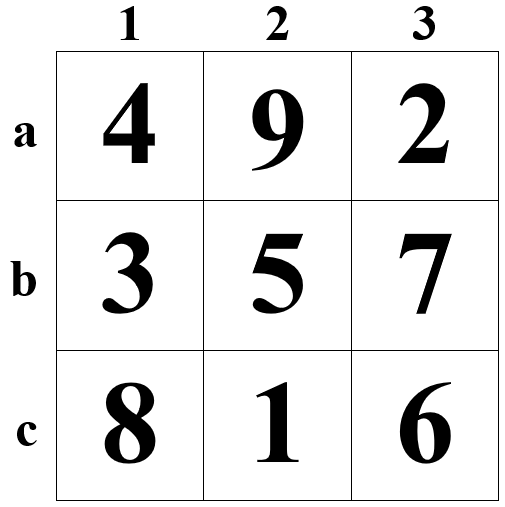
\includegraphics[width = 4cm]{images/Yupik_Square-solved.png}}
     
\item $456 = 20\times (20+2)+15+1 =$ \cmubdata{yuinaat yuinaq malruk akimiaq atauciq}
\end{solutions}

\rules Numbers are written in base 20. Numbers smaller than 20 are written as $10 + A$ or $15 + A$ (where $A$ is 1, 2, 3, or 4). Numbers smaller than 400, i.e., $20A + B$, are written as \cmubdata{yuinaat} $A$ $B$, where $A$ and $B$ are between 1 and 19.

\pagebreak
Base words are:
\begin{enumerate}[leftmargin = 5em, label = \arabic*]

    \begin{multicols}{2}
    \item \cmubdata{atauciq}
    \item \cmubdata{malruk}
    \item \cmubdata{pingayun}
    \item \cmubdata{cetaman}
    \item \cmubdata{talliman} (given in intro)
    \item \cmubdata{arvinlegen} (given in intro)
    \item \cmubdata{malrunglegen}
    \item[10] \cmubdata{qula}
    \item[15] \cmubdata{akimiaq}
    \item[20] \cmubdata{yuinaq} (\texttr{20+}), \cmubdata{yuinaat} (\texttr{20\times})
        \end{multicols}
\end{enumerate}

\noindent Addition is implicit and the constituent order is from big to small. For numbers bigger than 800, a new structure is added at the beginning -- \cmubdata{yuinaat yuinaak} $X$, meaning $400X$, and the rest is written as above. For example, $951 = 800 + 151 = (20\times20\times2) + (20\times7) + 11 =$ \texttr{(20\times) (20\times) (2) (20\times) (7) (10) (1)} = \cmubdata{yuinaat yuinaak malruk yuinaat malrunglegen qula atauciq}.
\end{mysolution}

\section{Overcounting}

\begin{problem}{\langnameUmbuUngu}{\nameKGilyarova}{\LOYear{\IOLAbbr}{2012}}
\hfill
\begin{tabular}[t]{cl}
    \lsptoprule
      & \langnameUmbuUngu \\\midrule              
    10 & \cmubdata{rureponga talu}    \\ 
    15 & \cmubdata{malapunga yepoko}  \\ 
    20 & \cmubdata{supu}              \\ 
    21 & \cmubdata{tokapunga telu}    \\ 
    27 & \cmubdata{alapunga yepoko}   \\ 
    30 & \cmubdata{polangipunga talu} \\ 
    \lspbottomrule
\end{tabular}\hfill
\begin{tabular}[t]{cl}
        \lsptoprule
        &   \langnameUmbuUngu\\\midrule
     35 & \cmubdata{tokapu rureponga yepoko} \\
     40 & \cmubdata{tokapu malapu} \\ 
     48& \cmubdata{tokapu talu} \\ 
     50& \cmubdata{tokapu alapunga talu} \\ 
     69& \cmubdata{tokapu talu tokapunga telu} \\ 
     79& \cmubdata{tokapu talu polangipunga yepoko} \\ 
     97& \cmubdata{tokapu yepoko alapunga telu} \\ 
     \lspbottomrule
\end{tabular}\hfill\hbox{}

\begin{tblsWarning}
    \cmubdata{telu < yepoko}
\end{tblsWarning}

\pagebreak
\begin{assgts}
\item \taskWriteNumbers:
\begin{enumerate}[label = \alph*.]
    \item \cmubdata{tokapu polanigpu}
    \item \cmubdata{tokapu talu rureponga telu}
    \item \cmubdata{tokapu yepoko malapunga talu}
    \item \cmubdata{tokapu yepoko polangipunga telu}
\end{enumerate}
\item \taskWriteIn{\langnameUmbuUngu}: 13, 66, 72, 76, 95.
\end{assgts}
\end{problem}

\begin{mysolution}
Initial observations:
\begin{itemize}
    \item \cmubdata{supu} is a single word, so most likely is a multiple of the base; therefore the base can be 4, 5, 10, or 20;
    \item 10 is not a single word, so it is unlikely that the base is 5, 10 or 20. Therefore, it seems to be a base-4 language;
    \item \cmubdata{tokapu} occurs in the number 35 (but it does not occur in 30), so it most likely means 32. 31, 33 and 34 do not seem to make sense as single words, since they are extremely unlikely as bases, and it can't be 35 either since there are other words following it. Moreover, 32 confirms the hypothesis that the language is base-4, since it is a multiple of 4;
    \item General structure: (\cmubdata{tokapu}) ($X$) ($Y$\cmubdata{-pu(nga)}) ($Z$).
\end{itemize}

 Based on this structure, we can count the digits. These appear as $X$ or $Z$ (but we notice that they do not occur as $Y$, which means that $Y$\cmubdata{-pu(nga)} is a single word). There are only three words appearing in $X$ and $Z$ positions: \cmubdata{talu}, \cmubdata{telu}, \cmubdata{yepoko}.

Moreover, we notice that 48 is \cmubdata{tokapu talu}. Most likely, \cmubdata{talu} is a multiplier for \cmubdata{tokapu}, and, since the numbers smaller than 48 do not contain this structure, we deduce that \cmubdata{talu} = 2. Indeed, for numbers 35 and 40, \cmubdata{tokapu} occurs without a multiplier (1 is implicit), so the first multiplier that ought to appear is 2. Based on the same logic, \cmubdata{yepoko} must mean 3 and, knowing that \cmubdata{telu} $<$ \cmubdata{yepoko}, we get that \cmubdata{telu} is 1.

Replacing these numbers in the given data, we get:

\begin{center}
\hfill
\begin{tabular}[t]{cl}
\lsptoprule
       & \langnameUmbuUngu                \\\midrule
    10 & \cmubdata{rureponga} 2   \\
    15 & \cmubdata{malapunga} 3   \\
    20 & \cmubdata{supu}          \\
    21 & \cmubdata{tokapunga} 1   \\
    27 & \cmubdata{alapunga} 3    \\
    30 & \cmubdata{polangipunga} 2\\
\lspbottomrule
\end{tabular}\hfill
\begin{tabular}[t]{cl}
\lsptoprule
   & \langnameUmbuUngu \\  \midrule
35 & \cmubdata{tokapu rureponga} 3 \\
40 & \cmubdata{tokapu malapu} \\
48 & \cmubdata{tokapu} 2 \\
50 & \cmubdata{tokapu alapunga} 2 \\
69 & \cmubdata{tokapu} 2\cmubdata{tokapunga} 1 \\
79 & \cmubdata{tokapu} 2 \cmubdata{polangipunga} 3 \\
97 & \cmubdata{tokapu} 3 \cmubdata{alapunga} 1 \\
\lspbottomrule
\end{tabular}
\hfill\hbox{}
\end{center}

 Based on the number 48, since we assumed that 2 is a multiplier, we deduce that \cmubdata{tokapu} = 24. Moreover, based on the first column, by subtraction, we obtain the numbers: \cmubdata{rureponga} = 8, \cmubdata{malapunga} = 12, \cmubdata{supu} = 20, \cmubdata{tokapunga} = 20, \cmubdata{alapunga} = 24, \cmubdata{polangipunga} = 28.

However, we notice that we have two different words for 20. Nevertheless, all words than end in \cmubdata{-punga} also have a units digit (1, 2 or 3), so it is possible that each word has two forms, one for when it appears alone and the other that appears when a units digit is added.
Thus, based on the words we know already, 35 is written as \texttr{24 8 3} (and, indeed, $35 = 24 + 8 + 3$).

An interesting thing happens with the number 40. Knowing that \cmubdata{tokapu} = 24, it must be that \cmubdata{malapu} is 16 (but we also know that \cmubdata{malapunga} = 12). Thus, we deduce the following rule: each multiple of 4 is a single or base word (ending in \cmubdata{-pu}). When a units digit (1, 2, or 3) is added, the following multiple of 4 is used to which the suffix \cmubdata{-nga} is added. Therefore, 24 = \cmubdata{tokapu} and 28 = \cmubdata{alapu}, but 25 = \cmubdata{alapunga telu} (basically, $(28-4) + 1$), 26 = \cmubdata{alapunga talu} ($28-4 + 2$) and 27 = \cmubdata{alapunga yepoko} ($28-4 + 3$).

This is a rather common phenomenon called \OlympiadNewTerm{overcounting}, in which the numbers are regarded as \textit{going towards...}. Thus, 27 can be translated literally as \texttr{three (units) towards 28} (meaning that it is three units past 24). Overcounting occasionally occurs Indo-European languages as well (e.g., in German, the clock time 7.30 is read as \cmubdata{halb acht} (meaning \texttr{half eight}) – which is to say, half an hour has passed \textit{towards 8 o'clock}).

A last observation concerns the numbers 48, 50 and 69. We notice that both 48 and 69 use the structure \cmubdata{tokapu talu} (meaning 48), but 50 does not, so we deduce that 50 is written as $24 + (28-4) + 2$. This can also be considered a type of overcounting. Normally, when “units”\ get as big as the order, we carryover and increase the multiplier by a unit (e.g., in English after \cmubdata{twenty-nine}, we do not say *\cmubdata{twenty-ten}, but rather \cmubdata{thirty}). In this language, however, the change of the order only occurs at 32 (although the base is 24). An indication pointing towards this is that, although we have single words for all multiples of 4, we do not have a word for 8 (thus, we cannot write the numbers 5, 6 and 7). For this reason, instead of writing $24X + 6$, we actually write $24(X-1) + 30$.

Based on all these observations, we can solve the tasks and write the solution:

\begin{solutions}
    \item
    \begin{enumerate}[label = \alph*., noitemsep]
        \item $24 + 32 = 56$
        \item $24\times2 + (12-4) + 1 = 57$
        \item $24\times3 + (16-4) + 2 = 86$
        \item $24\times3 + (32-4) + 1 = 101$
    \end{enumerate}
\end{solutions}

\note{In an official solution, it suffices to write just the number (the final result). Nevertheless, writing the structure formed by each morpheme is a safety net to prevent careless mistakes. The same goes for task (b).} 

\begin{solutions}[resume]
    \item 
    \begin{enumerate}[noitemsep,leftmargin=0pt]
    \item[] $13 = 12 + 1 = (16-4) + 1 =$ \cmubdata{malapunga telu}
    \item[] $66 = 24\times2 + 16 + 2 = (24\times2) + (20-4) + 2 =$ \cmubdata{tokapu talu supunga talu}
    \item[] $72 = 24\times3 =$ \cmubdata{tokapu yepoko}
    \item[] $76 = 24\times2 + 28 =$ \cmubdata{tokapu telu alapu}
    \item[] $95 = 24\times3 + 20 + 3 = (24\times3) + (24-4) + 3 =$ \cmubdata{tokapu yepoko tokapunga yepoko}
    \end{enumerate}
\end{solutions}

\rules

\begin{itemize}
    \item Base words ($X$): 1 = \cmubdata{telu}, 2 = \cmubdata{talu}, 3 = \cmubdata{yepoko}
    \item Base words ($Y$): 12 = \cmubdata{rurepo}, 16 = \cmubdata{malapu}, 20 = \cmubdata{supu}, 24 = \cmubdata{tokapu}, 28 = \cmubdata{alapu}, 32 = \cmubdata{polangipu}
    \item Addition is implicit.
    \item Numbers from 9 to 31 are written as: $Y$\cmubdata{-nga} $X = (Y-4) + X$.
    \item Numbers greater than 32, having the structure $24A + B$, are written as \cmubdata{tokapu} $A$ $B$, where $A = \{2, 3\}$, and $B$ is between 9 and 32 (except for 24, in which case it is directly written as $24(X+1)$ – in the data, 48 is not written as *\cmubdata{tokapu tokapu}, but rather \cmubdata{tokapu talu}).
\end{itemize}
\end{mysolution}

\begin{problem}{\langnameHuli}{\nameBHuang}{\LOYear{\UKLOAbbr}{2016}}
The perfect squares from 1 to 100 are written in Huli below, \OlympiadRandomOrder{}:

\begin{enumerate}[label = \Alph*., leftmargin = 1in]
    \item \cmubdata{ngui ki, ngui tebone-gonaga waragaria}
    \item \cmubdata{mbira}
    \item \cmubdata{ngui dau, ngui waragane-gonaga waragaria}
    \item \cmubdata{nguira-ni pira}
    \item \cmubdata{nguira-ni mbira}
    \item \cmubdata{dira}
    \item \cmubdata{maria}
    \item \cmubdata{ngui tebo, ngui mane-gonaga maria}
    \item \cmubdata{ngui ma, ngui dauni-gonaga maria}
    \item \cmubdata{ngui waraga, ngui kane-gonaga pira}
\end{enumerate}

\begin{assgts}
\item For each of them, write its corresponding value. 
\item Here are four consecutive numbers written in Huli, in ascending order:
\begin{enumerate}[label = \alph*.]
    \item \cmubdata{ngui ka, ngui haline-gonaga bearia}
    \item \cmubdata{ngui ka, ngui haline-gonaga hombearia}
    \item \cmubdata{ngui ka, ngui haline-gonaga haleria}
    \item \cmubdata{ngui ka, ngui haline-gonaga deria}
\end{enumerate}
\item[] Write their corresponding values.
\item \taskWriteIn{\langnameHuli}: 2, 4, 6, 7, 22, 44, 66, 77, 88, 173.
\end{assgts}
\end{problem}

\begin{mysolution}

 The first step is figuring out the structure of Huli numbers. We have three types of structures: single words (\cmubdata{dira}, \cmubdata{maria}, \cmubdata{mbira}), structures like \cmubdata{nguira-ni} $X$ and structures like \cmubdata{ngui} $X$, \cmubdata{ngui} $Y$\cmubdata{-gonaga} $Z$. At first sight, we would expect the numbers represented by single words to be the smallest (digits) – taking this with a grain of salt, since some of them could also represent orders, e.g., 100; numbers like \cmubdata{nguira-ni} $X$ are the second smallest ones (we can probably assimilate them with the type $base + X$), while the last category represents the biggest numbers ($base \times A + B$) – although we still do not know why there are three digits in these structures and not only two.

Once the structures are identified, we know exactly where the digits are placed in these structures, so we can try counting them in order to get an estimate of the base. We get the morphemes: \cmubdata{ki}, \cmubdata{tebone}, \cmubdata{waragaria}, \cmubdata{mbira}, \cmubdata{dau}, \cmubdata{waragane}, \cmubdata{pira}, \cmubdata{dira}, \cmubdata{maria}, \cmubdata{tebo}, \cmubdata{mane}, \cmubdata{ma}, \cmubdata{dauni}, \cmubdata{waraga}, \cmubdata{kane}. Nevertheless, we notice that digits can have different forms (since we find the triplets \cmubdata{ma -- mane -- maria} and \cmubdata{waraga -- waragane -- waragaria}, each of them following the same pattern: $X$ – $X$\cmubdata{-ne} -- $X$\cmubdata{-ria}), and furthermore, those without any suffix appear only after \cmubdata{ngui}, those with the suffix \cmubdata{-ne} appear only with the ending \cmubdata{-gonaga}, while those with the suffix \cmubdata{-ra/-ria} appear only at the very end, after \cmubdata{nguira-ni} or if they are single structures. Therefore, we can assume that they denote the same digit, and each digit has three different forms, depending on the context. Thus, we are left with 10 morphemes: \cmubdata{ki}, \cmubdata{mbi(ra)}, \cmubdata{dau}, \cmubdata{pi(ra)}, \cmubdata{di(ra)}, \cmubdata{dau(ni)}, \cmubdata{ka(ne)}, \cmubdata{tebo}, \cmubdata{waraga}, \cmubdata{ma}, so we could expect this language to be base-10. Nevertheless, if we look at task (b), we notice four more morphemes occur: \cmubdata{bea(ria)}, \cmubdata{hombea(ria)}, \cmubdata{hale(ria)}, \cmubdata{de(ria)}. Therefore, the total number of digits is 14. Since base 13 is extremely unlikely, as well as base 14, it is most likely one of the bases 12, 15 or 16 (among which, base 15 is the most likely one since we have discovered 14 morphemes).

Furthermore, since the base is bigger than 12, we certainly know that 1, 4, and 9 are digits (so they will be represented by a single word). Therefore, based on the previous observation according to which $X <$ \cmubdata{nguira-na} $X <$ \cmubdata{ngui} $X$\cmubdata{, ngui} $Y$\cmubdata{-gonaga} $Z$, we can already split the numbers into categories. Thus:

\exrule{
\{\cmubdata{mbira}, \cmubdata{dira}, \cmubdata{maria}\} must correspond to \{1, 4, 9\} -- the use of curly brackets shows that we are not sure about the exact order,}
and
\exrule{\{\cmubdata{nguira-ni mbira}, \cmubdata{nguira-ni pira}\} = \{16, 25\}.
}

Since \cmubdata{mbira} appears in both structures, we can try obtaining (by subtraction) the value of \cmubdata{nguira-ni}, which, most likely, represents the base.

We can do this by considering all the possible cases, as follows, and calculating the difference between them:

\begin{table}[H]
    \begin{tabular}{lc ccc}
         \lsptoprule
         & & \multicolumn{3}{c}{\cmubdata{mbira}} \\\cmidrule{3-5}
         & & {1} & {4} & {9} \\\cmidrule{3-5}
         \cmubdata{nguira-ni} & {16} & 15 & 12 & 7 \\
         \cmubdata{mbira} & {25} & 24 & 21 & 16 \\
         \lspbottomrule
    \end{tabular}
\end{table}

 Thus, the values for \cmubdata{nguira-ni}, and, implicitly, for the base are 7, 12, 15, 16, 21, 24. Since we know we have roughly 14 digits, we can exclude the bases 7, 21 and 24. Moreover, since 16 appears in the corpus (and it is not a single word), it is unlikely that it will be the base (if \cmubdata{nguira-ni} = 16, it follows that either \cmubdata{mbira} or \cmubdata{pira} is 0, which is impossible). So, we are left with the bases 12 and 15.

\begin{table}[H]
    \begin{tabular}{lc ccc}
         \lsptoprule
         & & \multicolumn{3}{c}{\cmubdata{mbira}} \\\cmidrule{3-5}
         & & {1} & {4} & {9} \\\cmidrule{3-5}
         \cmubdata{nguira-ni} & {16} & 15 & 12 &  \\
         \cmubdata{mbira} & {25} &  &  &  \\
         \lspbottomrule
    \end{tabular}
\end{table}

 Moreover, we notice that these two bases are possible only if \cmubdata{nguira-ni mbira} is 16. Thus, we already have the first two correspondences: \cmubdata{nguira-ni mbira} = 16, \cmubdata{nguira-ni pira} = 25. Moreover, if \cmubdata{nguira-ni} is 12, then \cmubdata{pira} must be 13, which is highly unlikely, since it would be greater than the base. Therefore, \cmubdata{nguira-ni} = 15 (we therefore talk about a base-15 system), \cmubdata{mbira} = 1, \cmubdata{pira} = 10.

Now we can analyse the more complex numbers (which we know most likely will be written as $15X + Y$). The first step is now writing the remaining squares like this (in order to make comparisons easier):


\begin{multicols}{3}
    \begin{itemize}

        \item[] $36 = 15\times2 + 6$
        \item[] $49 = 15\times3 + 4	$
        \item[] $64 = 15\times4 + 4$
        \item[] $81 = 15\times5 + 6$
        \item[] $100 = 15\times6 + 10$
    \end{itemize}
\end{multicols}

 Knowing that \cmubdata{pira} = 10, and 4 can only be \cmubdata{maria} or \cmubdata{dira}, we notice that these two occur multiple times at the end of some numbers, so we can group them like this:

\begin{table}[H]
    \begin{tabular}{r@{~=~}ll}
    36  & $15\times2 + 6$ & \cmubdata{ngui ki, ngui tebone-gonaga waragaria} \\
    81  & $15\times5 + 6$ & \cmubdata{ngui dau, ngui waragane-gonaga waragaria} \\\midrule
    49  & $15\times3 + 4$ & \cmubdata{ngui tebo, ngui mane-gonaga maria} \\
    64  & $15\times4 + 4$ & \cmubdata{ngui ma, ngui dauni-gonaga maria} \\\midrule
    100 & $ 15\times6 + 10$ & \cmubdata{ngui waraga, ngui kane-gonaga pira} \\
    \end{tabular}
\end{table}

 The numbers from the same cell are not necessarily ordered (i.e., we know that 36 and 81 are represented by the two phrases on the right, but we don't know which is which). Moreover, we deduce that \cmubdata{maria} = 4 (and we are left with \cmubdata{dira} = 9, since it is the only unassigned single word in the data) and \cmubdata{waragaria} = 6. Moreover, knowing that the numbers change their form $X$ -- $X$\cmubdata{-ne} -- $X$\cmubdata{-ria}, we can check if any of these numbers occur in any other position. At this stage, we can already replace them in the data. Last but not least, we can delete the units in order to simplify the table.
 
\begin{center}
    \begin{tabular}{ll@{~}l}
    $15\times2$ & \cmubdata{ngui ki,} &\cmubdata{ngui tebone-gonaga}  \\
    $15\times5$ & \cmubdata{ngui dau,} &\cmubdata{ngui \makebox[\widthof{tebone}][c]{6}-gonaga}  \\
    \midrule
    $15\times3$ & \cmubdata{ngui tebo,} &\cmubdata{ngui \makebox[\widthof{dauni}][c]{4}-gonaga}   \\
    $15\times4$ & \cmubdata{ngui \makebox[\widthof{tebo}][c]{4},} &\cmubdata{ngui dauni-gonaga}  \\
    \midrule
    $15\times6$ & \cmubdata{ngui \makebox[\widthof{tebo}][c]{6},} &\cmubdata{ngui kane-gonaga} \\
    \end{tabular}
\end{center}

Based on the last example (100), we notice that the first digit, after \cmubdata{ngui}, represents the multiplier of the base. Therefore, we deduce that \cmubdata{tebo} = 3, and we can make the correspondences in the second row:

\begin{center}
    \begin{tabular}{ll@{~}l}
    $15\times2$ & \cmubdata{ngui ki,} &\cmubdata{ngui tebone-gonaga}  \\
    $15\times5$ & \cmubdata{ngui dau,} &\cmubdata{ngui \makebox[\widthof{tebone}][c]{6}-gonaga}  \\
    \midrule
    $15\times3$ & \cmubdata{ngui \makebox[\widthof{dau}][c]{3},} &\cmubdata{ngui \makebox[\widthof{dauni}][c]{4}-gonaga}   \\
    \midrule
    $15\times4$ & \cmubdata{ngui \makebox[\widthof{dau}][c]{4},} &\cmubdata{ngui dauni-gonaga}  \\
    \midrule
    $15\times6$ & \cmubdata{ngui \makebox[\widthof{dau}][c]{6},} &\cmubdata{ngui kane-gonaga} \\
    \end{tabular}
\end{center}

 Furthermore, the number after \cmubdata{ngui} and the units are enough to calculate any number, so what could be the role of \cmubdata{ngui} $Y$\cmubdata{-gonaga}? Firstly, since it does not offer any supplementary information (it is redundant, since the value of the number can be calculated without it and only based on \cmubdata{ngui} $X$ and $Z$), it is probably somehow connected to one of the other digits and, since it also starts with \cmubdata{ngui}, it is most likely related to $X$. Looking at the example $15\times3$, we notice that $Y$ is 1 unit greater than $X$. Therefore, we deduce that $15X + Z$ is written in Huli as \cmubdata{ngui} $X$\cmubdata{, ngui} $(X+1)$\cmubdata{-gonaga} $Z$, and we can then determine all the correspondences:

\begin{solutions}
    \item \quad
    \begin{multicols}{5}
    \begin{enumerate}[label = \Alph* --]
        \item 36
        \item 1
        \item 81
        \item 25
        \item 16
        \item 9
        \item 4
        \item 49
        \item 64
        \item 100
    \end{enumerate}
    \end{multicols}
\end{solutions}

Moreover, we can make a table with the three different forms of the digits we have. Since this is base 15, we expect to have \textit{units} from 1 to 14:

\begin{table}[H]
    \begin{tabular}{ cccc }
    \lsptoprule
        Digits & units ($X$) & \cmubdata{ngui} $X$ & \cmubdata{ngui} $X$\cmubdata{-gonaga} \\
        \midrule
        1&\cmubdata{mbira} & & \\
        2& & \cmubdata{ki} & \\
        3& & \cmubdata{tebo} & \cmubdata{tebone} \\
        4&\cmubdata{maria} &\cmubdata{ma} &\cmubdata{mane} \\
        5& &\cmubdata{dau} &\cmubdata{dauni} \\
        6& \cmubdata{waragaria}&\cmubdata{waraga} &\cmubdata{waragane} \\
        7& &\cmubdata{ka} &\cmubdata{kane} \\
        8& & &\cmubdata{haline} \\
        9&\cmubdata{dira} & & \\
        10&\cmubdata{pira} & & \\
        11& & & \\
        12& & & \\
        13& & & \\
        14& & & \\
    \lspbottomrule
    \end{tabular}
\end{table}


\begin{solutions}[resume]
\item In task (b), we are given four extra consecutive numbers, and all of their unit digits are new (they do not occur anywhere else in the problem). Looking at the table above, the only four consecutive digits that do not occur anywhere else are 11--14, and, knowing that the numbers are in ascending order, we deduce that: \cmubdata{ngui ka, ngui haline-gonaga bearia} $= 7\times15 + 11 = 116$ and the other numbers are 117, 118, and 119 respectively.
\end{solutions}

Now we can fill in the table with the additional information:

 \begin{table}[H]
    \begin{tabular}{ cccc }
    \lsptoprule
        Digits & units ($X$) & \cmubdata{ngui} $X$ & \cmubdata{ngui} $X$\cmubdata{-gonaga} \\
        \midrule
        1&\cmubdata{mbira} & & \\
        2& & \cmubdata{ki} & \\
        3& & \cmubdata{tebo} & \cmubdata{tebone} \\
        4&\cmubdata{maria} &\cmubdata{ma} &\cmubdata{mane} \\
        5& &\cmubdata{dau} &\cmubdata{dauni} \\
        6& \cmubdata{waragaria}&\cmubdata{waraga} &\cmubdata{waragane} \\
        7& &\cmubdata{ka} &\cmubdata{kane} \\
        8& & &\cmubdata{haline} \\
        9&\cmubdata{dira} & & \\
        10&\cmubdata{pira} & & \\
        11&\cmubdata{bearia} & & \\
        12&\cmubdata{hombearia} & & \\
        13&\cmubdata{haleria} & & \\
        14&\cmubdata{deria} & & \\
    \lspbottomrule
    \end{tabular}
\end{table}

 The last thing we need to do is analyse the way in which the three forms are constructed. We notice that the second column (\cmubdata{ngui} $X$) is the base form and, in order to obtain the first column, we add the suffixes \cmubdata{-ra/-ira}, while the suffixes \cmubdata{-ne/-ni} are used to form the third column.

Analysing the occurrence of the suffix \cmubdata{-ra}, we realise that it is only used if the base form ends in \cmubdata{i}. So we can write the phonological rule: \mbox{\cmubdata{-ria \rightarrow~-ra / i \_ }}. For the last column, things are a bit more complicated since there is only one instance in which \cmubdata{ni} appears (with \cmubdata{dau}). Since we have only one example, it is hard to define a precise phonological rule. One option is to consider that \cmubdata{ni} appears after \cmubdata{u}, in which case we would talk about an assimilation of the vowel height, since both \cmubdata{i} and \cmubdata{u} are high vowels.

Thus, we can solve task (c).

\begin{solutions}[resume]
    \item
    \begin{enumerate}
        \item[2] = \cmubdata{kiria}
        \item[4] = \cmubdata{maria}
        \item[6] = \cmubdata{waragaria}
        \item[7] = \cmubdata{karia}
        \item[22] = \cmubdata{nguira-ni karia}
        \item[44] = \cmubdata{ngui ki, ngui tebone-gonaga deria}
        \item[66] = \cmubdata{ngui ma, ngui dauni-gonaga waragaria}
        \item[77] = \cmubdata{ngui dau, ngui waragane-gonaga kiria}
        \item[88] = \cmubdata{ngui dau, ngui waragane-gonaga haleria}
        \item[173] = \cmubdata{ngui bea, ngui hombeane-gonaga halira}
    \end{enumerate}
\end{solutions}

\rules
\begin{itemize}

    \item \cmubdata{nguira-ni} $X_2 = 15 + X$
    \item \cmubdata{ngui} $X_1$\cmubdata{, ngui} $(X_3 + 1)$\cmubdata{-gonaga} $Y_2 = 15X + Y$
    \item Subscripts 1, 2 and 3 denote the form of the digit:
    \begin{itemize}

        \item Form 2 -- base form;
        \item Form 1 -- add the suffix \cmubdata{-ria} (\mbox{\cmubdata{-ria \rightarrow~-ra / i \_ }});
        \item Form 3 -- add the suffix \cmubdata{-ne} (\mbox{\cmubdata{-ne \rightarrow~-ni / \{i, u\} \_ }});
    \end{itemize}
\end{itemize}
\end{mysolution}

 It is interesting to note the phenomenon in which we write both \cmubdata{ngui} $X$ and \cmubdata{ngui} $(X+1)$\cmubdata{-gonaga}, although the second part is redundant. Basically, we can consider this structure to mean $Z$ units after \cmubdata{ngui} $X$, towards \cmubdata{ngui} $(X+1)$-\cmubdata{gonaga}. For example, the number 49 (\cmubdata{ngui tebo, ngui mane-gonaga maria}) can be read as \texttr{four (units) away from the third group of 15s towards the fourth (group of 15s)}. This is another example of overcounting in which the units are enclosed between two consecutive multiples of the base.

\section{Subtractive systems}

 We have seen so far that the basic operations in every number system are addition and multiplication. There is, however, a special type of number system, subtractive systems, in which, besides addition and multiplication, subtraction also plays an important role. For example, in Problem 9.4, the numbers were formed as $M+1$, $M+2$, $M+3$, $N$ (where $M$ and $N$ are orders -- we ignore the fact that $M$ was derived from $N$). In subtractive systems, we can talk about numbers formed as \{$M$, $M+1$, $M+2$, $N-2$, $N-1$, $N$\} or \{$M$, $M+1$, $M+2$, $M+3$, $N-1$, $N$\}. Thus, 19 can, for example, be written as $20-1$ instead of $16+3$. It is important to not confuse subtractive systems with overcounting. In the case of overcounting, no subtraction is involved, but rather the order we use is one unit higher (since it is counted towards it), but still, the units are added. In subtractive systems, the units (or some of them) are subtracted from the order.

Currently, no purely subtractive system is known (in which addition does not play some role), and all subtractive systems use both addition and subtraction. Most subtractive systems only employ subtraction for 1 (therefore, for example, in such a base-10 subtractive system, the number 38 is written as $30 + 8$, but the number 39 is written as $40-1$).

\begin{problem}{\langnameYoruba}{\nameHSomers}{\LOYear{\UKLOAbbr}{2020}}
Here are some numbers in Yoruba:
\begin{center}
    \begin{tabular}{lr@{\hskip6em}lr}
         \pbsvnum{èji}{2} & \pbsvnum{\d{e}\d{\'{e}}rìndilogóji}{36} \\
         \pbsvnum{\d{\`{e}}rin}{4} & \pbsvnum{\d{\`{e}}rìndogóji}{44} \\
         \pbsvnum{àrun}{5} & \pbsvnum{àádorin}{70} \\
         \pbsvnum{\d{\`{e}}rinlá}{14} & \pbsvnum{\d{e}\d{\'{e}}tàdilogórin}{77} \\
         \pbsvnum{eéjìdilogun}{18} & \pbsvnum{\d{\`{e}}tàdogórin}{83} \\
    \end{tabular}
\end{center}

\begin{assgts}
\item \taskWriteNumbers:
\begin{multicols}{3}
\begin{enumerate}[label = \alph*.]
    \item \cmubdata{àádota}
    \item \cmubdata{àrùndogórin}
    \item \cmubdata{aárùndilogórin}
    \item \cmubdata{\d{\`{e}}tàdogórun}
    \item \cmubdata{òkándilogóji}
    \blankitem
\end{enumerate}
\end{multicols}
\item \taskWriteIn{\langnameYoruba}: 12, 45, 57, 90, 99.
\end{assgts}

\begin{tblsWarning}
The marks above the vowels denote tones; \cmubdata{e} and \cmubdata{\d{e}} are distinct vowels.
\end{tblsWarning}
\end{problem}

\begin{mysolution}

Firstly, we can notice the pair 4 and 14, in which the only difference is the suffix \cmubdata{-lá}. We can therefore deduce that $10 + X = X$\cmubdata{-lá}, so this system is most likely base-10.

Next, we have the pair 36 and 44, in which the only difference is \cmubdata{-il-}. Moreover, the first part of the word is highly similar to the word for 4 (in the case of 44 it is actually identical, while in the case of 36 it is slightly mutated), and the same thing goes for the pair 77 and 83. We notice that a common aspect of these numbers is that they are symmetrical with respect to the closest tens (thus, 36 and 44 are symmetrical with respect to 40, i.e., $36 = 40 - 4$ and $44 = 40 + 4$, while 77 and 83 are symmetrical with respect to 80, i.e. ±3). This can make us think of a subtractive system. Moreover, the last morpheme of 36 and 44 is \cmubdata{óji} (which resembles \cmubdata{èji} = 2), while the last morpheme of 77 and 83 is \cmubdata{órin} (\cmubdata{\sim ẹ̀rin}). Since this number cannot refer to the units (we know already that the units are 4 and 3, respectively), it most likely represents the tens. Thus, 40 = \cmubdata{óji}, and 80 = \cmubdata{órin}. Therefore, we realise it is actually a base-20 system, and the structure of the numbers is:

\begin{itemize}
    \item $X$\cmubdata{-lá} $= 10 + X$
    \item $U$\cmubdata{-dog-}$Z = 20Z + U$
	\item $U$\cmubdata{-dilog-}$Z = 20Z - U$
\end{itemize}

 Moreover, we notice that 70 has a special form, also derived from \cmubdata{órin} = 80, so, most probably, it represents $80 - 10$.

Thus, we notice that the digits have different forms depending on the context in which they appear (single units, $10 + X$, added units, subtracted units, $20X$, $20X-10$). Moreover, we already noticed that $10+X$ uses the same form of $X$ as the single unit, so we can combine these two forms.

Combining everything into a table, we get:

\begin{table}[H]
    \begin{tabular}{ *6{c} }
    \lsptoprule
    & Unit / $10+X$& $+$ units & $-$ units & $20X$ & $20X-10$\\
    \midrule
    1 & &  &  & \cmubdata{un} & \\
    2 & \cmubdata{èji}&  & \cmubdata{eéjì} & \cmubdata{óji} & \\
    3 & & \cmubdata{ẹ̀tà} & \cmubdata{ẹẹ́tà} &  & \\
    4 & \cmubdata{ẹ̀rin} & \cmubdata{ẹ̀rìn} & \cmubdata{ẹẹ́rìn} &  \cmubdata{órin} & \cmubdata{àádorin}\\
    5 & \cmubdata{àrun} &  &  &  & \\
    \lspbottomrule
    \end{tabular}
\end{table}

 Since we have all the different forms of the digit 4, we can see the transformations that take place. In order to form the added units, the second vowel receives a grave accent; to form the subtracted units, the first vowel is doubled (of which the first is toneless, while the second has an acute accent), and the final vowel gets a grave accent. In order to form $20X$, the first vowel becomes \cmubdata{ó}, while for the formation of $20X-10$, the first vowel is replaced by \cmubdata{àádo-}.

The only exception is the number 20 ($20\times1$), but, as explained before, we can expect that digit 1 might have some irregular forms.

 Another simpler way to write the rules is to notice that each digit has the structure \cmubdata{\`{V}\textsubscript{1}CV\textsubscript{2}(n)}. We can easily derive the rest of the forms: $+$ units = \cmubdata{\`{V}\textsubscript{1}C\`{V}\textsubscript{2}(n)}, $-$ units = \cmubdata{V\textsubscript{1}\'{V}\textsubscript{1}C\`{V}\textsubscript{2}(n)}, $20X$ = \cmubdata{ó CV\textsubscript{2}(n)}, $20X-10$ = \cmubdata{àádo CV\textsubscript{2}(n)}, once again, mentioning that for 1 the form $20X$ is irregular (\cmubdata{un}).

 Thus, we can solve all the tasks:

\begin{assgts}
    \item
    \begin{multicols}{5}
    \begin{enumerate}[label = \alph*.]

        \item 50
        \item 85
        \item 75
        \item 103
        \item 39
    \end{enumerate}
    \end{multicols}

\end{assgts}
\note{In order to figure out the meaning of \cmubdata{òkán} in task (e), we need to look at the table above (which we previously filled in with the additional information that we discovered in task (a)) and we notice that 1 is the only digit for which we do not know the subtracted units form (column 3 from the table above). So we can conclude that \cmubdata{òkán} is the subtracted form of 1. Moreover, we see again that its form is irregular.}

\begin{assgts}[resume]
    \item
    \begin{multicols}{2}
    \begin{enumerate}
        \item[12] = \cmubdata{èjilá}
        \item[90] = \cmubdata{àádorun}
        \item[57] = \cmubdata{ẹẹ́tàdilogóta}
        \item[45] = \cmubdata{àrùndogóji}
        \item[99] = \cmubdata{òkándilogórun}
        \item[]
    \end{enumerate}
    \end{multicols}
\end{assgts}
\end{mysolution}

\section{Body-part counting systems}

In this type of system, the names of the digits are derived from the names of body parts. Thus, 1 = \texttr{little finger}, 2 = \texttr{ring finger}, 3 = \texttr{middle finger}, 4 = \texttr{index finger}, 5 = \texttr{thumb}, 6 = \texttr{hand}, 7 = \texttr{elbow}, 8 = \texttr{arm}, 9 = \texttr{shoulder}, 10 = \texttr{ear}, 11 = \texttr{head}. Depending on the language, the number of body parts which are used can vary (some languages also include terms for \texttr{wrist}, \texttr{forearm}, \texttr{arm}, \texttr{eye}, etc.). We mentioned in the beginning of this chapter that the base of these systems is usually between 22 and 28. The interesting thing about these systems starts as soon as we reach the word for \texttr{head} (or \texttr{forehead}, \texttr{nose}, etc.), which represents the centre. From here on, the words are repeated in reverse order, with an additional morpheme/word which means \texttr{opposite/other}. Thus, continuing the series above, 12 = \texttr{opposite ear}, 13 = \texttr{opposite shoulder}, 14 = \texttr{opposite arm}, 15 = \texttr{opposite elbow}, 16 = \texttr{opposite hand}, 17 = \texttr{opposite thumb}, and so on.

At first sight, this particularity, although interesting, does not seem to pose any problems, but let us consider the following examples:
\ea Let us first consider a classic number system (not based on body parts) -- for example, Japanese -- and let us consider two pairs of numbers:

{\cmubdata{san} -- \cmubdata{juusan} and \cmubdata{go} -- \cmubdata{juugo}}
\z

In the case of these numbers, we have pairs following the pattern $X$ -- \cmubdata{juu-}$X$. So, if we are told that \cmubdata{san} = 3 and \cmubdata{juusan} = 13, we could instantly deduce that \cmubdata{juu-} = 10 (since $13 - 3 = 10$), and, if, additionally, we are told that \cmubdata{go} = 5, we will immediately claim that \cmubdata{juugo} = 15.

\ea Let us now consider a body-part-based system -- e.g., the Kombai system, used in New Guinea -- and let us analyse the following numbers:

{\cmubdata{woro} = 4, \cmubdata{imofo woro} = 20, \cmubdata{go} = 6, \cmubdata{imofo go} = ?}
\z

 If we followed the same method as in the previous case, we would again notice the pattern $X$ -- \cmubdata{imofo} $X$, and based on the pair 4 -- 20, we would deduce that \cmubdata{imofo} = 16, so we would say that \cmubdata{imofo go} = 22. Nevertheless, in reality, \cmubdata{imofo go} = 18, since the Kombai number system is based on body parts, centred on 12. Therefore, we notice that for these systems, the order is not obtained by subtracting two numbers like $X$ and \cmubdata{imofo} $X$, but rather by \emph{adding} them.

For Japanese: \cmubdata{juusan} $-$ \cmubdata{san} $= 10 =$ \cmubdata{juugo} $-$ \cmubdata{go}, but for Kombai \cmubdata{woro} $+$ \cmubdata{imofo woro} $=$ \cmubdata{go} $+$ \cmubdata{imofo go}. This is the main issue (and difficulty) with this type of system: the fact that it can easily be confused with a classic system, but, in fact, the base is obtained by adding two similar numbers rather than subtracting them.

A separate discussion concerns what one considers to be the base of such a system. We return to the example of Kombai, where we mentioned that the system is ``centred on 12'', but \cmubdata{imofo go} + \cmubdata{go} = 24. For linguistics problems, it is preferred that the base is considered as the double of the centre, because, in this way, we will have the relation \cmubdata{imofo} $X = 24 - X$. If we considered the base to be 12, the relation between the two numbers would become: $X = 12 - a$, while \cmubdata{imofo} $X = 12 + a$, which is much harder to use in practice.

\section{Time}

Problems related to time (reading the clock, calendar, etc.) can be considered a subtype of number systems since these problems will almost always feature numbers. It is rather common for the names of the days of the week and the months of the year to be formed based on numbers (\texttr{Monday} = day 1, \texttr{March} = month 3). This phenomenon is obvious in Chinese, where, starting from the numbers 1 = {\chinesetext{一}}, 2 = {\chinesetext{二}}, 3 = {\chinesetext{三}}, 4 = {\chinesetext{四}}, we can write the days of the week and the months as follows: \texttr{Monday} = {\chinesetext{星期一}}, \texttr{Tuesday} = {\chinesetext{星期二}}, \texttr{Wednesday} = {\chinesetext{星期三}}, \texttr{Thursday} = {\chinesetext{星期四}}; \texttr{January} = {\chinesetext{一月}}, \texttr{February} = {\chinesetext{二月}}, \texttr{March} = {\chinesetext{三月}}, \texttr{April} = {\chinesetext{四月}}.

Although these problems are relatively rare at the level of international linguistics competitions, they can feature some interesting phenomena, as shown in the following two problems.

\begin{problem}{\langnameCzech}{\nameMFried}{\PrincetonAbbr}
Here are some examples of how to tell the time in Czech:
\begin{center}
\begin{longtable}{ll}
\pbsv{za pět minut osm}{five minutes to eight} \\
\pbsv{za deset minut osm}{ten minutes to eight} \\
\pbsv{čtvrt na osm}{quarter past seven} \\
\pbsv{za sedm minut osm}{seven minutes to eight} \\
\pbsv{za osm minut čtvrt na osm}{seven minutes past seven} \\
\pbsv{za deset minut čtvrt na sedm}{five minutes past six} \\
\pbsv{půl osmé}{half past seven} \\
\pbsv{půl deváté}{half past eight} \\
\pbsv{za deset minut půl šesté}{twenty minutes to five} \\
\pbsv{čtvrt na deset}{quarter past nine} \\
\end{longtable}
\end{center}
\begin{assgts}
\item \transinen[\langnameCzech]
\begin{enumerate}
    \item \texttr{twenty-three minutes past five}
    \item \texttr{ten minutes to nine}
\end{enumerate}
\end{assgts}

\end{problem}

\begin{mysolution}

 We notice three types of structures:

\begin{itemize}
    \item \cmubdata{čtvrt na ...} = \texttr{quarter past ...}
    \item \cmubdata{půl ...-é} = \texttr{half past ...}
    \item \cmubdata{za ... minut (čtvrt na / půl) ...} -- otherwise
 \end{itemize}

 It is obvious that \wordtrans{minut}{minute(s)}, so if we compare the first two examples, we obtain: \cmubdata{osm} = 8, \cmubdata{deset} = 10 and \cmubdata{pět} = 5. Moreover, we deduce that \cmubdata{za} $X$ \cmubdata{minut} $Y =$ \texttr{X minutes to Y}.

 We notice that \cmubdata{osm} occurs in the phrase \texttr{half past seven}, but not in \texttr{half past eight}. This indicates that Czech also features overcounting when it comes to telling the time (similar to German). Therefore, \cmubdata{půl} $X$\cmubdata{-é} = \texttr{half past $(X-1)$}, from which we deduce that \cmubdata{devát} = 9.

 Moreover, looking at the example \texttr{quarter past seven}, in which the word \cmubdata{osm} = 8 occurs again, we deduce that overcounting is also applied for quarters, so \cmubdata{čtvrt na} $X$ = \texttr{quarter past $(X-1)$} (or \texttr{quarter towards X}).

 The only structures we are left to analyse are those following the pattern \cmubdata{za} $X$ \cmubdata{minut ... na} $Y$. We can separate them from the rest and replace the words we already know:

 \begin{center}
     \begin{tabular}{ll}
          \pbsv{za osm minut čtvrt na osm}{seven minutes past seven}\\
          \pbsv{za deset minut čtvrt na sedm}{five minutes past six}\\
          \pbsv{za deset minut půl šesté}{twenty minutes past five}\\
     \end{tabular}
 \end{center}

 We already know that the hour is placed in the end, so we can directly replace the structures \cmubdata{čtvrt na} $X$ and \cmubdata{půl šesté}. Moreover, we know all the words, so we notice that \texttr{seven minutes past seven} is written as \cmubdata{za} \texttr{8 minutes quarter past seven}, and \texttr{five minutes past six} is written as \cmubdata{za} \texttr{10 minutes quarter past six}. We therefore notice that the Czech system is based on overcounting. Therefore, \texttr{seven minutes past seven} is translated as \texttr{8 minutes to [quarter towards 8]} or \texttr{8 minutes to [quarter past 7]}.

 The same thing is noticed in the structure \cmubdata{za deset minut půl šesté} which is literally translated as \texttr{10 minutes to [half towards 6]} or \texttr{10 minutes to [half past 5]}.

 So we now know all the possible structures so we can write the rules and solve the tasks.

 \rules

 \begin{itemize}

     \item \cmubdata{půl} $X$\cmubdata{-é} = \texttr{half past $(X-1)$} 
     \item \cmubdata{čtvrt na} $X$ = \texttr{quarter past $(X-1)$} 
     \item \cmubdata{za} $X$ \cmubdata{minut} $Y$ = \texttr{$X$ minutes to $Y$}, where $Y$ can be a full hour (o'clock) or any of the two structures above.
 \end{itemize}

 \begin{assgts}
     \item 1. \texttr{23 past 5} = \texttr{7 minutes to [half past five]} = \texttr{7 minutes to [half towards 6]} = \cmubdata{za sedm minut půl šesté}
     \item[] 2. \texttr{10 past 9} = \texttr{5 minutes to [quarter past nine]} = \texttr{5 minutes to [quarter towards 10]} = \cmubdata{za pět minut čtvrt na deset}
 \end{assgts}

 In this case, overcounting is used for all the structures, but, as mentioned above, there are languages in which only certain structures use overcounting. For example, in German, overcounting is only used in the half-past constructions -- \cmubdata{halb} $X$ = \texttr{half past $(X-1)$}.
\end{mysolution}

 \begin{problem}{\langnameSwahili}{\nameNSarda}{\LOYear{\PLOAbbr}{2014}}
Here are some Swahili phrases and their English translations \OlympiadRandomOrder{}:

\begin{table}[H]
    \begin{tabular}{rl@{\hskip0.3in}cl}
        \chaosline{jumamosi, saa moja usiku}{Sunday, 1.00 AM}
        \chaosline{jumapili, saa tatu na robu asubuhi}{Sunday, 7.30 AM}
        \chaosline{jumamosi, saa saba usiku}{Sunday, 9.15 AM}
        \chaosline{jumamosi, saa mbili na robu usiku}{Tuesday, 12.15 PM}
        \chaosline{jumanne, saa tano na nusu usiku}{Tuesday, 11.30 PM}
        \chaosline{jumanne, saa sita na robu asubuhi}{Saturday, 10.30 AM}
        \chaosline{jumamosi, saa nne na nusu asubuhi}{Saturday, 7.00 PM}
        \chaosline{jumapili, saa moja na nusu asubuhi}{Saturday, 8.15 PM}
    \end{tabular}
\end{table}

\begin{assgts}
\item \detcorr
\item \transinen
\begin{enumerate}[start = 9]
    \item \cmubdata{jumatano, saa moja na robu asubuhi}
    \item \cmubdata{jumapili, saa nne na nusu asubuhi}
\end{enumerate}
\pagebreak
\item \transinen[\langnameSwahili]
\begin{multicols}{2}
\begin{enumerate}[start = 11]
    \item \texttr{Monday, 12.15 AM}
    \item \texttr{Monday, 10.00 PM}
\end{enumerate}
\end{multicols}
\end{assgts}
\end{problem}

\begin{mysolution}

 The first step is noticing the structure of the phrases. All of them start with a word separated by a comma, which has the prefix \cmubdata{juma-}. This most likely represents the day (it is unlikely that all that variety of times would use the same one-word structure). Therefore, the structure after the comma must be the time. For this, we notice two types of structures:

\exrule{\cmubdata{saa} $X$ \cmubdata{usiku} \quad\quad and \quad\quad \cmubdata{saa} $X$ \cmubdata{na \{robu/nusu\} \{usiku/asubuhi\}}}

 We can assume that the simplest structure refers to the o'clock times, which is also reinforced by the fact that we only have two such structures in both Swahili and English. Thus:

\begin{center}
    \begin{tabular}{ll}

    \pbsv{jumamosi, saa moja usiku}{Sunday, 1.00 AM} \\
    \pbsv{jumamosi, saa saba usiku}{Saturday, 7.00 PM} \\
    \end{tabular}
\end{center}

Curiously, in Swahili, the same name seems to be used to express different days in English. We will have to explain why that is in due course.

Among the remaining examples, only one more contains the hour 7 (although it is AM, instead of PM), and only one other example starts with either \cmubdata{saa saba} or \cmubdata{saa moja} (since we do not know the correspondence between the two). Since phrase 8 contains \cmubdata{saa moja}, we deduce that it corresponds to translation B. Moreover, we deduce that \cmubdata{saa moja} means 7 o'clock, so we can make three correspondences:

\begin{center}
    \begin{tabular}{rl@{\hskip1em}cl}
         1. & \cmubdata{jumamosi, saa moja usiku} & G. & \texttr{Saturday, 7.00 PM}\\
         3. & \cmubdata{jumamosi, saa saba usiku} & A. & \texttr{Sunday, 1.00 AM}\\
         8. & \cmubdata{jumapili, saa moja na nusu asubuhi} & B. & \texttr{Sunday, 7.30 AM}\\
    \end{tabular}
\end{center}

 Based on example 8, we can infer that \cmubdata{na nusu} means \texttr{half past}. Moreover, most likely, \cmubdata{usiku} and \cmubdata{asubuhi} correspond, in some way, to the notion of AM and PM, but it is not a one-to-one correspondence, since \cmubdata{usiku} is used for both 7 PM and 1 AM.

We only have two more examples which contain \cmubdata{na nusu} (5 and 7), and the English times correspond to 10.30 AM and 11.30 PM. Since \cmubdata{usiku} is used for both 7 PM and 1 AM, we can assume that it will also be used for 11.30 PM, so that \cmubdata{usiku} suggests the idea of \texttr{evening/night}.

	We get two more correspondences:

\begin{center}
    \begin{tabular}{rl@{\hskip1em}cl}
         1. & \cmubdata{jumamosi, saa moja usiku} & G. & \texttr{Saturday, 7.00 PM}\\
         3. & \cmubdata{jumamosi, saa saba usiku} & A. & \texttr{Sunday, 1.00 AM}\\
         8. & \cmubdata{jumapili, saa moja na nusu asubuhi} & B. & \texttr{Sunday, 7.30 AM}\\
         5. & \cmubdata{jumanne, saa tano na nusu usiku} & E. & \texttr{Tuesday, 11.30 PM}\\
         7. & \cmubdata{jumamosi, saa nne na nusu asubuhi} & F. & \texttr{Saturday, 10.30 AM}\\
    \end{tabular}
\end{center}

 The last three correspondences can be easily made. Only one of the phrases contains the word \cmubdata{usiku}, and among the times 8.15 PM, 9.15 AM, 12.15 PM, the only one that refers to evening time is 8.15 PM. Therefore, 4=H. Among the remaining two phrases, one starts with \cmubdata{jumanne}, which seems to mean \texttr{Tuesday}. Therefore, we have the correspondences:

\begin{center}
    \begin{tabular}{rl@{\hskip1em}cl}
         1. & \cmubdata{jumamosi, saa moja usiku} & G. & \texttr{Saturday, 7.00 PM}\\
         3. & \cmubdata{jumamosi, saa saba usiku} & A. & \texttr{Sunday, 1.00 AM}\\
         8. & \cmubdata{jumapili, saa moja na nusu asubuhi} & B. & \texttr{Sunday, 7.30 AM}\\
         5. & \cmubdata{jumanne, saa tano na nusu usiku} & E. & \texttr{Tuesday, 11.30 PM}\\
         7. & \cmubdata{jumamosi, saa nne na nusu asubuhi} & F. & \texttr{Saturday, 10.30 AM}\\
         2. & \cmubdata{jumapili, saa tatu na robu asubuhi} & C. & \texttr{Sunday, 9.15 AM}\\
         4. & \cmubdata{jumamosi, saa mbili na robu usiku} & H. & \texttr{Saturday, 8.15 PM}\\
    \end{tabular}
\end{center}

 To sum up, we notice that \cmubdata{usiku} is used between 7 PM and 1.00 AM (it corresponds to \texttr{evening/night}), while \cmubdata{asubuhi} is used between 7.30 AM and 12.15 PM (it corresponds to \texttr{morning/day}).

One of the issues we noticed in the beginning was that the Swahili days of the week do not match the English ones. So let us separate (and order chronologically) these dates:

\begin{center}
    \begin{tabular}{rl@{\hskip1em}cl}
        6. & \cmubdata{jumanne, saa sita na robu asubuhi} & D. & \texttr{Tuesday, 12.15 PM}\\ 5. & \cmubdata{jumanne, saa tano na nusu usiku} & E. & \texttr{Tuesday, 11.30 PM}\\
        \midrule
        7. & \cmubdata{jumamosi, saa nne na nusu asubuhi} & F. & \texttr{Saturday, 10.30 AM}\\
         1. & \cmubdata{jumamosi, saa moja usiku} & G. & \texttr{Saturday, 7.00 PM}\\
         4. & \cmubdata{jumamosi, saa mbili na robu usiku} & H. & \texttr{Saturday, 8.15 PM}\\
         3. & \cmubdata{jumamosi, saa saba usiku} & A. & \texttr{Sunday, 1.00 AM}\\
         \midrule
         8. & \cmubdata{jumapili, saa moja na nusu asubuhi} & B. & \texttr{Sunday, 7.30 AM}\\
         2. & \cmubdata{jumapili, saa tatu na robu asubuhi} & C. & \texttr{Sunday, 9.15 AM}\\
    \end{tabular}
\end{center}

 We notice that \cmubdata{jumanne} always corresponds to \texttr{Tuesday}, but \cmubdata{jumamosi} includes both \texttr{Saturday} and \texttr{Sunday}. Nevertheless, if we look closely, we notice that the Sunday phrase (which in Swahili is translated as \texttr{Saturday}) has the time 1.00 AM. Therefore, we deduce that, in Swahili, the day does not change at midnight, but rather when \cmubdata{usiku} ends. So, according to the data given, the day starts and ends when evening becomes morning, some time after 1.00 AM and before 7.30 AM.

We can now compare the usage of numbers for day and hour. The only morpheme that is repeated is \cmubdata{nne} (meaning \texttr{Tuesday} and 10). Nevertheless, if we analyse the data closely, we also notice other pairs like \cmubdata{pili} -- \cmubdata{mbili} (\texttr{Sunday}, 8) and \cmubdata{mosi} -- \cmubdata{moja} (\texttr{Saturday}, 7). Thus, it seems like the Swahili week begins on Saturday, and the Xth day of the week is translated using the number $6+X$ (i.e., first day, Saturday, is translated using 7; day 2, Sunday, using 8, etc.).

Based on this, we can solve the tasks (b) and (c).\largerpage[2.5]

\begin{assgts}[resume]
    \item 9. \texttr{Wednesday, 7.15 AM}

    \noindent \cmubdata{jumatano} is formed from \cmubdata{tano} = 11, so it corresponds to \texttr{Wednesday}; \cmubdata{saa moja na robu asubuhi} = 7.15 AM.
    \item[] 10. \texttr{Sunday, 10.30 AM}
    \item 11. \cmubdata{jumapili, saa sita na robu usiku}

    \noindent Firstly, since the time is 12.15 AM, we know that in Swahili the day before will be used, hence, \texttr{Sunday}.
    \item[] 12. \cmubdata{jumatatu, saa nne usiku}
\end{assgts}

\rules
\begin{enumerate}
    \item General structure: \fbox{[\textit{Day of the week}], [\textit{Time}]}
    \item \fbox{[\textit{Time}]}: \cmubdata{saa} [X] [Y] [Z]
    \begin{itemize}
        \item[] X = hour
        \item[] Y: \wordtrans{na robu}{quarter past}, \wordtrans{na nusu}{half past}
        \item[] Z: \wordtrans{usiku}{night-time}, \wordtrans{asubuhi}{day-time}
    \end{itemize}
    \item
    \hfill\begin{tabular}[t]{r@{~}l l@{~}l}
        \lsptoprule
        \multicolumn{2}{l}{Hour} & \multicolumn{2}{l}{Day of the week} \\\midrule
        7 & \cmubdata{moja} & \cmubdata{jumamosi} & \texttr{Saturday} \\
        8 & \cmubdata{mbili} & \cmubdata{jumapili} & \texttr{Sunday} \\
        9 & \cmubdata{tatu} & \cmubdata{} & \texttr{Monday} \\
        10 & \cmubdata{nne} & \cmubdata{jumanne} & \texttr{Tuesday} \\
        11 & \cmubdata{tano} & \cmubdata{} & \texttr{Wednesday} \\
        12 & \cmubdata{sita} & \cmubdata{} & \texttr{Thursday} \\
        1 & \cmubdata{saba} & \cmubdata{} & \texttr{Friday} \\
        \lspbottomrule
    \end{tabular}\hfill\hbox{}
\end{enumerate}
\end{mysolution}

\begin{discussion}

 In reality, the Swahili system is much more interesting and simpler than it may seem. In countries where Swahili is spoken, the sun rises at around 7 AM so the people consider 7 AM to be the first hour of the day (8 AM is the second hour, etc.), and the sunrise is also the moment in which the day changes. The words \cmubdata{usiku} and \cmubdata{asubuhi} also refer strictly to sunrise and sunset (\cmubdata{usiku} = between 7 PM and 6.59 AM = \texttr{after sunset}, and \cmubdata{asubuhi} = between 7 AM and 6.59 PM = \texttr{after sunrise}).

Thus, the days of the week are named: day 1, day 2 etc. (first day is Saturday) and the table becomes:

\begin{table}[H]
    \begin{tabular}[t]{c@{~}ll@{~}l}
         \lsptoprule
        \multicolumn{2}{l}{Hour} & \multicolumn{2}{l}{Day of the week} \\
        \midrule
        1 & \cmubdata{moja} & \cmubdata{jumamosi} & \texttr{Saturday} \\
        2 & \cmubdata{mbili} & \cmubdata{jumapili} & \texttr{Sunday} \\
        3 & \cmubdata{tatu} & \cmubdata{} & \texttr{Monday} \\
        4 & \cmubdata{nne} & \cmubdata{jumanne} & \texttr{Tuesday} \\
        5 & \cmubdata{tano} & \cmubdata{} & \texttr{Wednesday} \\
        6 & \cmubdata{sita} & \cmubdata{} & \texttr{Thursday} \\
        7 & \cmubdata{saba} & \cmubdata{} & \texttr{Friday} \\
         \lspbottomrule 
         \multicolumn{4}{c}{\cmubdata{saa} $X = (X+6)$ \texttr{o'clock}}\\
    \end{tabular}
\end{table}

 This system of counting hours based on the sunrise is rather common in Equatorial Africa, where the day length is relatively constant, and a similar system is also used in Ethiopia. What is important to remember is that every language is used to express a culture and that culture might be completely different from yours. Therefore, when approaching a linguistics problem, it is important to keep an open mind and not expect all things to work in the way you are used to (e.g., the day changes at midnight, the numbers are in base 10, the week has 7 days, etc.).
\end{discussion}
\hypertarget{practice-problems}{%
\section{Practice problems}}

\begin{problem}{\langnameDanish}{\nameMSwan}{\LOYear{\UKLOAbbr}{2012}}
Here are some numbers written in Danish:
\begin{center}
    \begin{tabular}{lr@{\hskip6em}lr}
         \pbsvnum{tre}{3} & \pbsvnum{tredive}{30} \\[0.3em]
         \pbsvnum{fire}{4} & \pbsvnum{fyrre}{40} \\[0.3em]
         \pbsvnum{fem}{5} & \pbsvnum{syvoghalvtreds}{57} \\[0.3em]
         \pbsvnum{seks}{6} & \pbsvnum{tres}{60} \\[0.3em]
         \pbsvnum{syv}{7} & \pbsvnum{otteoghalvfjerds}{78} \\[0.3em]
         \pbsvnum{tyve}{20} & \pbsvnum{firs}{80} \\
    \end{tabular}
\end{center}

\begin{assgts}
\item \taskWriteNumbers:
\begin{multicols}{2}
\begin{enumerate}[label = \alph*.]
    \item \cmubdata{treogtyve}
    \item \cmubdata{seksoghalvtreds}
    \item \cmubdata{fireogtres}
    \item \cmubdata{femoghalvfjerds}
    \item \cmubdata{syvoghalvfems}
    \blankitem
\end{enumerate}
\end{multicols}
\item \taskWriteIn{\langnameDanish}: 8, 27, 36, 65, 98.
\end{assgts}

\end{problem}

\begin{problem}{\langnameEstonian}{\nameBNewsome}{\LOYear{\UKLOAbbr}{2014}}
The following expressions show how to tell the time in Estonian:

\begin{longtable}{ccc}
    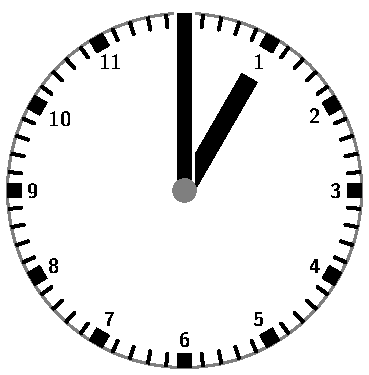
\includegraphics[width=3cm]{figures/Estonian_1.pdf} & 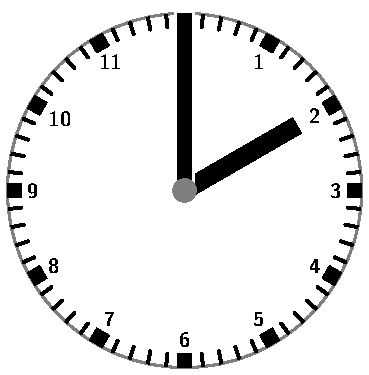
\includegraphics[width=3cm]{figures/Estonian_2.pdf} & 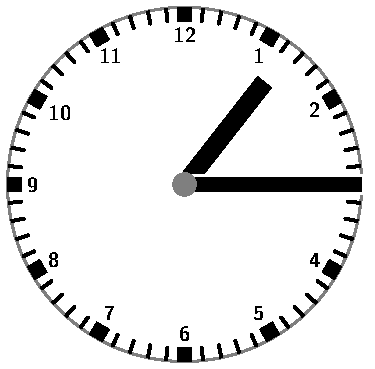
\includegraphics[width=3cm]{figures/Estonian_3.pdf} \\
    \cmubdata{Kell on üks} & \cmubdata{Kell on kaks} & \cmubdata{Veerand kaks} \\[0.8em]
    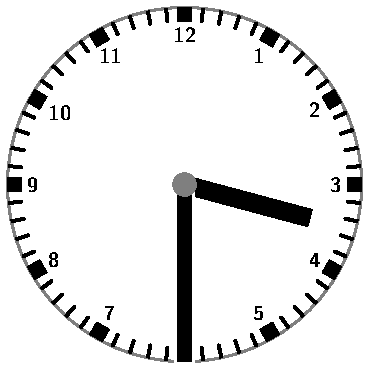
\includegraphics[width=3cm]{figures/Estonian_4.pdf} & 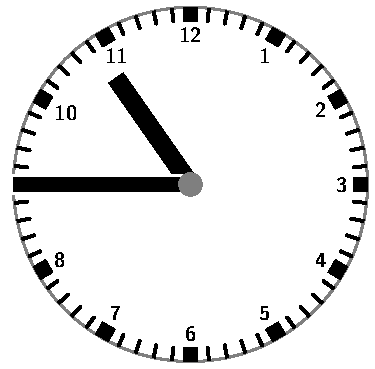
\includegraphics[width=3cm]{figures/Estonian_5.pdf} & 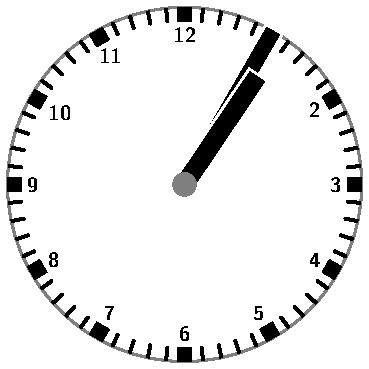
\includegraphics[width=3cm]{figures/Estonian_6.pdf} \\
    \cmubdata{Pool neli} & \cmubdata{Kolmveerand üksteist} & \cmubdata{Viis minutit üks läbi} \\
\end{longtable}

Here are some numbers in Estonian:
\begin{multicols}{5}
\begin{enumerate}[leftmargin = 0pt]
    \item[] 6 = \cmubdata{kuus}
    \item[] 7 = \cmubdata{seitse}
    \item[] 8 = \cmubdata{kaheksa}
    \item[] 9 = \cmubdata{üheksa}
    \item[] 10 = \cmubdata{kümme}
\end{enumerate}
\end{multicols}

\begin{assgts}
\item What do the following Estonian time expressions mean? Write with numbers:
\begin{enumerate}[label = \alph*.]
    \item \cmubdata{Kakskümmend viis minutit üheksa läbi}
    \item \cmubdata{Veerand neli}
    \item \cmubdata{Pool kolm}
    \item \cmubdata{Kolmveerand kaksteist}
    \item \cmubdata{Kolmkümmend viis minutit kuus läbi}
\end{enumerate}
\item Write the following times in Estonian:
\begin{multicols}{5}
\begin{enumerate}[label = \alph*., start = 6]
    \item 8:45
    \item 4:15
    \item 11:30
    \item 7:05
    \item 12:30
\end{enumerate}
\end{multicols}
\end{assgts}
\end{problem}

\begin{problem}{\langnameWaorani}{\nameDRadev}{\LOYear{\UKLOAbbr}{2012}}
Here are some equalities written in Waorani. Each sequence printed in bold represents one number from 1 to 10.

\begin{enumerate}[label=(\arabic*)]
\item \cmubdata{{mẽña mẽña mẽña mẽña} $+$ {mẽña go mẽña} $=$ {ãẽmãẽmpoke go aroke} $\times$ 2}
\item \cmubdata{{aroke}\textsuperscript{2} $+$ {mẽña}\textsuperscript{2} $=$ {ãẽmãẽmpoke}}
\item \cmubdata{{ãẽmãẽmpoke go aroke}\textsuperscript{2} $=$ {mẽña go mẽña} $\times$ {ãẽmãẽmpoke mẽña go mẽña}}
\item \cmubdata{{mẽña} $\times$ {ãẽmãẽmpoke} $=$ {tipãẽmpoke}}
\end{enumerate}

\begin{assgts}
\item Write in Waorani the numbers from 4 to 10.
\end{assgts}
\end{problem}

\pagebreak
\begin{problem}{\langnameSelkup}{\nameSBurlak}{\LOYear{\MSKAbbr}{1991}}
Here are some numbers in Selkup and their values \OlympiadRandomOrder{}: 

\begin{exe}
\sn[]{\cmubdata{somplylasar εj šitty}, \cmubdata{muktyssar εj ukkyr}, \cmubdata{sompylasar εj sompyla}, \cmubdata{šittysar}, \cmubdata{ukkyr ca muktyssar}, \cmubdata{šitty ca tɛ̄sar}, \cmubdata{sompylasar εj sel’cy}, \cmubdata{ukkyr ca tōn}
\glt 20, 38, 52, 55, 57, 59, 61, 99}
\end{exe}

\begin{assgts}
\item \detcorr
\item \taskWriteIn{\langnameSelkup}: 41, 48, 77, 98.
\end{assgts}

\begin{tblsWarning}
A bar above a vowel denotes length.
\end{tblsWarning}
\end{problem}

\begin{problem}{\langnameVambon}{\nameAPiperski}{\ElementyAbbr}
Below are given the following equalities written in Vambon \OlympiadRandomOrder{}: 
\begin{center}
    $3\times1 = 3$	\quad \quad\quad $3\times2 = 6$	\quad\quad \quad ...\quad \quad\quad 	$3\times9 = 27$
\end{center}
\begin{multicols}{2}
\begin{enumerate}
\itemsep0in
\item[] \cmubdata{takhem $\times$ ambalop $=$ emkelop}
\item[] \cmubdata{takhem $\times$ hitulop $=$ silutop}
\item[] \cmubdata{takhem $\times$ javet $=$ emsanop}
\item[] \cmubdata{takhem $\times$ kumuk $=$ emalin}
\item[] \cmubdata{takhem $\times$ mben $=$ emben}
\item[] \cmubdata{takhem $\times$ muyop $=$ emhitulop}
\item[] \cmubdata{takhem $\times$ sanop $=$ takhem}
\item[] \cmubdata{takhem $\times$ sanopkunip $=$ kumuk}
\item[] \cmubdata{takhem $\times$ takhem $=$ javet}
\blankitem
\end{enumerate}
\end{multicols}
\begin{assgts}
\item \taskWriteNumbers:
    \begin{enumerate}[label = \alph*.]
        \item (\cmubdata{emnggokmit} $+$ \cmubdata{nggokmit}) $\div$ \cmubdata{sanopkunip} $=$ \cmubdata{kalit}
        \item \cmubdata{emambalop} $-$ \cmubdata{emjavet} $=$ \cmubdata{hitulop}
    \end{enumerate}
\pagebreak
\item \taskWriteIn{\langnameVambon}:

\begin{multicols}{2}
    \begin{enumerate}[label = \alph*., start = 3]
        \item $20 + 22 - 26 = 16$
        \item $12 + 13 = 25$
    \end{enumerate}
\end{multicols}

\item You are given the following Vambon words:
\begin{center}
    \begin{tabular}{ll@{\hskip1in}ll}
         \pbsv{kalit}{nose} & \pbsv{kelop}{eye} \\[0.3em]
         \pbsv{kumuk}{wrist} & \pbsv{muyop}{elbow} \\[0.3em]
         \pbsv{nggokmit}{neck} & \pbsv{sanopkunip}{ring finger} \\[0.3em]
         \pbsv{silutop}{ear} &  \\
    \end{tabular}
\end{center}
\item[] Which body parts do the following words refer to?
\begin{multicols}{3}
 \begin{enumerate}[label = \alph*., start = 5]
        \item \cmubdata{ambalop}
        \item \cmubdata{javet}
        \item \cmubdata{malin}
        \item \cmubdata{mben}
        \item \cmubdata{sanop}
        \blankitem
    \end{enumerate}
\end{multicols}
\item What does the prefix \cmubdata{em-} mean in Vambon?
\end{assgts}
\end{problem}

\begin{problem}{\langnameAlamblak}{\nameRDinca}{\LOYear{\RoLOAbbr}{2013}}
Here are some Alamblak numbers and their numerical values \OlympiadRandomOrder{}:
\begin{enumerate}[leftmargin = 5em, label = \alph*.]
\itemsep0em
    \item \cmubdata{yima hosfirpati tir hosfirpat}
    \item \cmubdata{yima yohtti tir hosfi rpat}
    \item \cmubdata{yima hosfi hosf}
    \item \cmubdata{yima hosfi tir hosf}
    \item \cmubdata{yima yohtti tir yohtti rpat}
    \item \cmubdata{yima hosfirpati tir hosfi hosfirpat}
    \item \cmubdata{yima hosfirpati tir hosfirpati hosfirpat}
    \item \cmubdata{yima yohtti tir hosfirpati rpat}
    \item \cmubdata{yima hosfihosfi tir yohtti hosfihosf}
    \item \cmubdata{yima hosfi tir hosfi hosf}
%     \blankitem
\end{enumerate}

\begin{center}
    26, 31, 36, 42, 50, 52, 73, 75, 78, 89
\end{center}\pagebreak

Moreover, it is known that: 
\begin{center}

\begin{tabular}{llll}
    $1 =$ \cmubdata{rpat}	& $2 =$ \cmubdata{hosf}	 & $3 =$ \cmubdata{hosfirpat} & $4 =$ \cmubdata{hosfihosf} \\[0.3em]		
    $5 =$ \cmubdata{tir yohtt} & $6 =$ \cmubdata{tir yohtti rpat} & \multicolumn{2}{l}{11 = \cmubdata{tir hosfi rpat}}\\
\end{tabular}
\end{center}

\begin{assgts}
\item \detcorr
\item \taskWriteNumbers:
\begin{enumerate}[label = \alph*., start = 11]
   \item \cmubdata{yima hosfirpati hosfihosf} + \cmubdata{yima yohtti tir hosf} = \\ \hspace*{\fill} = \cmubdata{yima hosfihosfi tir hosfi hosfihosf} 
    \item \cmubdata{tir yohtti hosf} + \cmubdata{tir hosfi hosf} = \cmubdata{tir hosfirpati hosfihosf}
\end{enumerate}
\item \taskWriteIn{\langnameAlamblak}: 21, 48, 83.
\end{assgts}
\end{problem}

\begin{problem}{\langnameChabu}{\nameDMysak}{\LOYear{\UkrLOAbbr}{2018}}
Below are given the first four multiples of the number \cmubdata{efi tʃumtʃum eku bab eku iŋki}, written in Chabu in ascending order (if the number is X, the four numbers below represent 2X, 3X, 4X, and 5X, respectively):
\begin{enumerate}
    \item[] \cmubdata{bab ef eku efi tʃumtʃum eku iŋki}
    \item[] \cmubdata{ink ufe kor eku bab eku bab}
    \item[] \cmubdata{ink ufe kor eku bab ef eku bab}
    \item[] \cmubdata{bab ufe kor}
\end{enumerate}
\begin{assgts}
\item Write in Chabu all the divisors of the number \cmubdata{bab eku iŋki ufe kor} (including 1). If you consider some of them can be written in different ways, write all the possibilities. 
\end{assgts}
\end{problem}

\begin{problem}{\langnameTifal}{\nameSBurlak\ \& \namePArkadiev}{\LOYear{\MSKAbbr}{2017}}
Here are some equalities written in Tifal. It is known that none of the numbers in the problem are greater than 30. 
\begin{multicols}{2}
\begin{enumerate}[leftmargin = 1em]
\itemsep0in
\item[] \cmubdata{asumano $\times$ aleeb $=$ bokob}
\item[] \cmubdata{asumano $\times$ ataling $=$ tadang}
\item[] \cmubdata{bokob $\times$ ataling $=$ ataling madi}
\item[] \cmubdata{bokob $\times$ asumano $=$ nakal madi}
\item[] \cmubdata{asumano $\times$ feet $=$ feet madi}
\item[] \cmubdata{ataling $\times$ ataling $=$ tadang madi}
\item[] \cmubdata{asumano $+$ ataling $=$ feet}
\item[] \cmubdata{feet $+$ miit $=$ feet madi}
\item[] \cmubdata{tadang $+$ ataling $=$ tadang madi}
\blankitem
\end{enumerate}
\end{multicols}
\begin{assgts}
\item \taskWriteNumbers:
\begin{enumerate}[label = (\arabic*)]
    \item \cmubdata{beeti $+$ nakal $=$ beeti madi}
    \item \cmubdata{bokob $+$ maakob $=$ feet}
    \item \cmubdata{awok $\times$ awok $=$ asumano madi}
\end{enumerate}
\item Write in Tifal the results of the following equalities:
\begin{enumerate}[label = (\arabic*), start = 4]
    \item \cmubdata{tadang $+$ miit $=$}
    \item \cmubdata{ataling madi $-$ aleeb $=$}
\end{enumerate}
\end{assgts}
\end{problem}

\begin{problem}{\langnameMansi}{\nameIDerzhanski}{\LOYear{\IOLAbbr}{2005}}
Here are some numbers in Mansi (written in Latin script): 
\begin{center}
\begin{tabular}{lr}
     \pbsvnum{ńollow}{8} \\[0.3em]
     \pbsvnum{atxujplow}{15} \\[0.3em]
     \pbsvnum{atlow nopъl ontъllow}{49} \\[0.3em]
     \pbsvnum{atlow}{50} \\[0.3em]
     \pbsvnum{ontъlsāt ontъllow}{99} \\[0.3em]
     \pbsvnum{xōtsātn xōtlow nopъl at}{555} \\[0.3em]
     \pbsvnum{ontъllowsāt}{900} \\[0.3em]
     \pbsvnum{ontъllowsāt ńollowxujplow}{918} \\[0.3em]
\end{tabular}
\end{center}
\begin{assgts}
\item \taskWriteNumbers:

\begin{enumerate}[label = \alph*.]
    \setlength{\multicolsep}{6.0pt plus 2.0pt minus 1.5pt}
    \begin{multicols}{2}   
    \item \cmubdata{atsātn at}
    \item \cmubdata{ńolsāt nopъl xōt}
    \end{multicols}
    \item \cmubdata{ontъllowsātn ontъllowxujplow}
\end{enumerate}
\item \taskWriteIn{\langnameMansi}: 58, 80, 716.
\end{assgts}
\end{problem}

\hypertarget{solutions-of-practice-problems}{%
\section{Solutions of practice problems}}

\begin{practiceproblemsolution}{9.9. \langnameDanish}

\begin{solutions}[label=Solution 9.9\alph*]
    \item
    \begin{multicols}{5}
        \begin{enumerate}[label = \alph*.]
            \item 23
            \item 56
            \item 64
            \item 75
            \item 97
        \end{enumerate}
    \end{multicols}
    {\item \setlength\columnsep{-1em}
    \begin{multicols}{3}
    \setlength\columnsep{-2em}
        \begin{enumerate}
            \item[8] = \cmubdata{otte}
            \item[27] = \cmubdata{syvogtyve}
            \item[36] = \cmubdata{seksogtredive}
            \item[65] = \cmubdata{femogtres}
            \item[98] = \cmubdata{otteoghalvfems}
        \end{enumerate}
    \end{multicols}}
\end{solutions}

\rules

 The Danish system is based on \textit{scores} (20s) rather than \textit{tens}, thus: \cmubdata{tres} (3) \rightarrow \cmubdata{treds} ($20 \times 3 = 60$); \cmubdata{fire} (4) \rightarrow \cmubdata{firs} ($20 \times 4 = 80$). Note that there are special words for  20, 30, and 40.

The particle \cmubdata{halv-} attached before means $-10$ (\texttr{halfway towards}), while noting that the word might undergo some phonological changes (\cmubdata{tres -- treds}, \cmubdata{firs -- fjerds}): \cmubdata{treds} (60) \rightarrow \cmubdata{halvtreds} ($60 - 10 = 50$).

The numbers are formed following the structure $U$\cmubdata{og}$S$ ($U$ represents units and $S$ scores; \cmubdata{og} means \texttr{and}).
\end{practiceproblemsolution}


\begin{practiceproblemsolution}{9.10. \langnameEstonian}

\begin{solutions}[label=Solution 9.10\alph*]
    \item
    \begin{multicols}{5}
        \begin{enumerate}[label = \alph*.]
            \item 9:25
            \item 3:15
            \item 2:30
            \item 11:45
            \item 6:35
        \end{enumerate}
    \end{multicols}
    \item
    \begin{multicols}{2}
        \begin{enumerate}[label = \alph*., start = 6]
            \item \cmubdata{kolmveerand üheksa}
            \item \cmubdata{veerand viis}
            \item \cmubdata{pool kaksteist}
            \item \cmubdata{viis minutit seitse läbi}
            \item \cmubdata{pool üks}
            \item[]
        \end{enumerate}
    \end{multicols}
\end{solutions}

\rules \quad
\begin{multicols}{2}
    \begin{itemize}
        \item X:00 = \cmubdata{kell on} X
        \item X:15 = \cmubdata{veerand} (X+1)
        \item X:30 = \cmubdata{pool} (X+1)
        \item X:45 = \cmubdata{kolmveerand} (X+1)
        \item Else, X:Y = Y \cmubdata{minutit} X \cmubdata{läbi}
        \item $10+X$ = X-\cmubdata{teist}
        \item $10X+Y$ = X-\cmubdata{kümmend} Y
        \item[]
		\end{itemize}
\end{multicols}

\end{practiceproblemsolution}
\pagebreak
\begin{practiceproblemsolution}{9.11. \langnameWaorani}

\begin{solutions}[label=Solution 9.11\alph*]
    \item
    \begin{multicols}{2}
    \begin{enumerate}[label = \arabic* =, start = 4]
        \item \cmubdata{mẽña go mẽña}
        \item \cmubdata{ãẽmãẽmpoke}
        \item \cmubdata{ãẽmãẽmpoke go aroke}
        \item \cmubdata{ãẽmãẽmpoke go mẽña}
        \item \cmubdata{mẽña mẽña mẽña mẽña}
        \item \cmubdata{ãẽmãẽmpoke mẽña go mẽña}
        \item \cmubdata{tipãẽmpoke}
        \item[]
    \end{enumerate}
    \end{multicols}
\end{solutions}
\end{practiceproblemsolution}

\begin{practiceproblemsolution}{9.12. \langnameSelkup}

\begin{solutions}[label=Solution 9.12\alph*]
\item
    \begin{tabular}[t]{@{}l@{~}l  l@{~}l@{}}
         \cmubdata{somplylasar εj šitty} & = 52 & \cmubdata{muktyssar εj ukkyr} & = 61\\
         \cmubdata{sompylasar εj sompyla} & = 55 & \cmubdata{šittysar} & = 20\\
         \cmubdata{ukkyr ca muktyssar} & = 59 & \cmubdata{šitty ca tɛ̄sar} & = 38\\
         \cmubdata{sompylasar εj sel’cy} & = 57 & \cmubdata{ukkyr ca tōn} & = 99\\
    \end{tabular}
    \item
    \begin{tabular}[t]{@{} ll @{}}
         41 = \cmubdata{tɛ̄sar εj ukkyr}  & 48 = \cmubdata{šitty ca sompylasar} \\
         77 = \cmubdata{sel’cysar εj sel’cy} & 98 = \cmubdata{šitty ca tōn} \\
    \end{tabular}
\end{solutions}

\rules
\begin{itemize}
    \item Base-10 subtractive system.
    \item $10X = X$\cmubdata{-sar}	\hfill	100 = \cmubdata{tōn}
    \item $10X + Y = X$\cmubdata{-sar εj} $Y$ \hfill $Y = (1,7)$
    \item $10X + Y = (10-Y)$ \cmubdata{ca} $(X+1)$\cmubdata{-sar} \hfill $Y=(8,9)$
\end{itemize}
\end{practiceproblemsolution}

\begin{practiceproblemsolution}{9.13. \langnameVambon}

 Body-part-based system, centred on 14.

\begin{solutions}[label=Solution 9.13\alph*]
    \item a. $(17+11) \div 2 = 14$ \quad\quad\quad\quad\quad\quad  b. $23-19=4$
    \item c. \cmubdata{emuyop + emkumuk – emsanopkunip = emsilutop}
    \itemsep0in
    \item[] d. \cmubdata{silutop + kelop = emtakhem}
    \item
    \begin{multicols}{3}
        \begin{enumerate}[label = \alph*., start = 5,leftmargin = 1em]

            \item \texttr{thumb}
            \item \texttr{arm}
            \item \texttr{shoulder}
            \item \texttr{forearm}
            \item \texttr{little finger}
            \item[]
        \end{enumerate}
    \end{multicols}
    \item The prefix \cmubdata{em-} means \texttr{other / opposite}. Note: \cmubdata{em \rightarrow~e / \_ m}.
\end{solutions}
\end{practiceproblemsolution}

\begin{practiceproblemsolution}{9.14. \langnameAlamblak}
\begin{solutions}[label=Solution 9.14\alph*]
    \item
    \begin{multicols}{5}

        \begin{enumerate}[label = \alph*.]
            \item 71
            \item 31
            \item 42
            \item 50
            \item 26
            \item 73
            \item 78
            \item 36
            \item 89
            \item 52
        \end{enumerate}
    \end{multicols}
    \item k. $64+30=97$ \quad\quad\quad\quad\quad\quad l. $7+12=19$
    \item 21 = \cmubdata{yima yohtti rpat}
    \item[] 48 = \cmubdata{yima hosfi tir yohtti hosfirpat}
    \item[] 83 = \cmubdata{yima hosfihosfi hosfirpat}
\end{solutions}

\rules
\begin{itemize}
    \item General structure: \cmubdata{yima} $X$\cmubdata{-i tir} $Y$\cmubdata{-i} $Z = 20X + 5Y + Z$
    \item The digit 1 has two different forms: \cmubdata{rpat} (if it is $Z$), \cmubdata{yohtti} (for $X$ or $Y$)
    \item Thus, multiplication is implied, while addition is marked by the suffix \cmubdata{-i}
\end{itemize}
\end{practiceproblemsolution}

\begin{practiceproblemsolution}{9.15. \langnameChabu}

\begin{solutions}[label=Solution 9.15\alph*]
    \item
    \begin{multicols}{2}
        \begin{enumerate}
            \item \cmubdata{iŋki / ink}
            \item \cmubdata{bab}
            \item \cmubdata{bab eku iŋki}
            \item \cmubdata{bab eku bab}
            \item \cmubdata{efi tʃumtʃum}
            \item \cmubdata{efi tʃumtʃum eku iŋki}
            \item[10] \cmubdata{bab ef}
            \item[12] \cmubdata{bab ef eku bab}
            \item[15] \cmubdata{bab ef eku efi tʃumtʃum}
            \item[20] \cmubdata{ink ufe kor}
            \item[30] \cmubdata{ink ufe kor eku bab ef}
            \item[]
        \end{enumerate}
    \end{multicols}
\end{solutions}

\rules
\begin{enumerate}
    \item General structure:
\begin{itemize}
    \item $2 [+ X] =$ \cmubdata{bab} $[$\cmubdata{eku} $X] \hfill (X < 3)$
    \item $5 [+ X] =$ \cmubdata{efi tʃumtʃum} $[$\cmubdata{eku} $X] \hfill (X < 5)$
    \pagebreak
    \item $10 [+ X] =$ \cmubdata{bab ef} $[$\cmubdata{eku} $X] \hfill (X < 10)$
    \item $20Y [+ X] =$ $Y$ \cmubdata{ufe kor} $[$\cmubdata{eku} $X] \hfill (X < 20)$
\end{itemize}
\item $Y$ is written even if it is 1 (20 = \cmubdata{ink ufe kor}).
\item The digit 1 has two forms: \cmubdata{ink} (if it is a multiplier) or \cmubdata{iŋki} (if it is added). In task (a), 1 has two alternative spellings, since we do not know which one to choose if it appears as a single word.
\end{enumerate}
\end{practiceproblemsolution}

\begin{practiceproblemsolution}{9.16. \langnameTifal}

\begin{solutions}[label=Solution 9.16\alph*]
    \item
    \begin{enumerate}[label = (\arabic*)]
        \item $9+10=19$
        \item $6+1=7$
        \item $5\times5=25$
    \end{enumerate}
    \item
    \begin{enumerate}[label = (\arabic*), start = 4]
        \item \cmubdata{tadang $+$ miit $=$ aleeb madi}
        \item \cmubdata{ataling madi $–$ aleeb $=$ bokob madi}
    \end{enumerate}
\end{solutions}

\rules

Body-part-based system, centred on 14.  $X$ \cmubdata{madi} $= 28 – X$.
\end{practiceproblemsolution}



\begin{practiceproblemsolution}{9.17. \langnameMansi}

\begin{solutions}[label=Solution 9.17\alph*]
    \item
       \begin{multicols}{3}
    \begin{enumerate}[label = \alph*., leftmargin = 1em]
        \item 405
        \item 76
        \item 819
    \end{enumerate}
    \end{multicols}
    \item 58 = \cmubdata{xōtlow nopъl ńollow}
    \item[] 80 = \cmubdata{ńolsāt}
    \item[] 716 = \cmubdata{ńollowsātn xōtxujplow}
\end{solutions}

\begin{sloppypar}
\rules System based largely on overcounting. Tens are formed from units: adding the suffix \cmubdata{-low} (for 50, 60) or replacing the suffix \cmubdata{-low} with \cmubdata{-sāt} (for 80, 90).
\end{sloppypar}

\begin{multicols}{2}
    \begin{itemize}

        \item[] $10 + X = X$\cmubdata{-xujplow}
        \item[] $10X + Y = 10(X+1)$ \cmubdata{nopъl} $Y$
        \item[] $90 + X =$ \cmubdata{ontъlsāt} $X$
        \item[] $100X = X$\cmubdata{-sāt}
        \item[] $100X + Y = (X+1)$\cmubdata{-sātn} $Y$
        \item[] $900 + X =$ \cmubdata{ontъllowsāt} $X$
    \end{itemize}
\end{multicols}
\end{practiceproblemsolution}

% \section{Further reading}
% \begin{enumerate}[{label=[\arabic{*}]}]
%     \item Chrisomalis, Stephen. “Numerical notation: a comparative history.”\ \textit{Cambridge University Press}, Cambridge (2010).
%     \item Hurford, James R. “The linguistic theory of numerals.”\ \textit{Cambridge University Press}, Cambridge (2011).
%     \item Ifrah, George. “The universal history of numbers: from prehistory to the invention of the computer.”\ \textit{John Wiley and Sons Inc.}, New York (2000).
%     \item Zaslavsky, Claudia. “Africa counts: number and pattern in African cultures.”\ \textit{Chicago Review Press}, Chicago (1999).
% \end{enumerate}

\nocite{Chrisomalis2010, Hurford2011, Ifrah2000, Zaslavsky1999}
% \printbibliography[heading=FurtherReading]
\FurtherReadingBox{}
\end{refsection}
